\chapter{Introduction}

\section{Alzheimer's Disease (AD)}

Alzheimer’s disease (AD\nomenclature{AD}{Alzheimer's disease}) is a devastating neurodegenerative disorder, clinically characterised by progressive memory loss, cognitive decline, and behavioural impairment. The most common form of dementia, it is estimated to affect 50 million people worldwide with numbers expecting to triple to 152 million by 2050, ensuing both a heavy global economic and social burden amounting to over US\$1 trillion annually\cite{International2020}. Despite international efforts to better understand the disorder for drug discovery and development, there is currently no cure and existing medication only act to ameliorate symptoms.

\subsection{Pathology}
The symptoms of AD are underpinned by both morphological and molecular changes in the brain. Neuroimaging and post-mortem brain analysis from patients reveal significant brain atrophy caused by neuronal and synaptic loss\cite{Selkoe1991,Perl2010} (\cref{fig:AD_intro}). Further microscopic examination has revealed the accumulation of beta-amyloid (A$\beta$) in amyloid plaques (\cref{fig:AD_development}\textbf{a}) and the aggregation of tau in neurofibrillary tangles (NFT\nomenclature{NFT}{Neurofibrillary tangles}) (\cref{fig:AD_development}\textbf{b}), two key hallmarks of AD, which are now believed to manifest years before presentation of clinical symptoms and diagnosis \cite{Sperling2011}. These neuropathological changes are accompanied with heightened neuroinflammation through the abnormal activation and distribution of microglia (the most abundant brain resident immune cells) and astrocytes (glial cells with multiple roles in supporting neuronal function and metabolism) \cite{Heneka2015}. 

The progression of these neuropathological changes have been well mapped in post-mortem tissue, particularly the spread of NFTs which is quantified using Braak staging\cite{H1991} (\cref{fig:AD_development}\textbf{c}). Pathology is initially apparent in the temporal lobes (hippocampus and entorhinal cortex) and later spreads to the frontal lobes. Conversely, the occipital lobes, motor cortex, and the cerebellum are relatively resistant to neuronal degeneration even in advanced stages of AD\cite{Xu2019}.

% Protein aggregates a common feature of neurodegenerative diseases; tie in AD with other dementias
Of note, it is important to emphasise that aside from A$\beta$ deposition and NFT formation, 15-20\% of AD patients also have evidence of Lewy body (LB) pathology \cite{C1995,L2003} - the defining pathological hallmark of Parkinson's disease (PD)\cite{Wakabayashi2007}\nomenclature{PD}{Parkinson's Disease} and dementia with Lewy bodies (DLB)\cite{Spillantini1997}\nomenclature{DLB}{Dementia with Lewy Bodies}. This is characterised by abnormal aggregation of $\alpha$-synuclein into intra-neuronal cytoplasmic inclusion bodies. Up to 75\% of AD patients further present neuronal cytoplasmic inclusions comprising of aggregates of TDP-43 \cite{King2010,McAleese2017,Arai2009} (Transactive response DNA binding protein-43), the defining hallmarks of frontotemporal dementia (FTD\nomenclature{FTD}{Frontotemporal dementia}) and amyotrophic laternal sclerosis\cite{Pesiridis2009} (ALS\nomenclature{ALS}{amyotrophic laternal sclerosis}).

\begin{figure}[!htp]
	\centering
	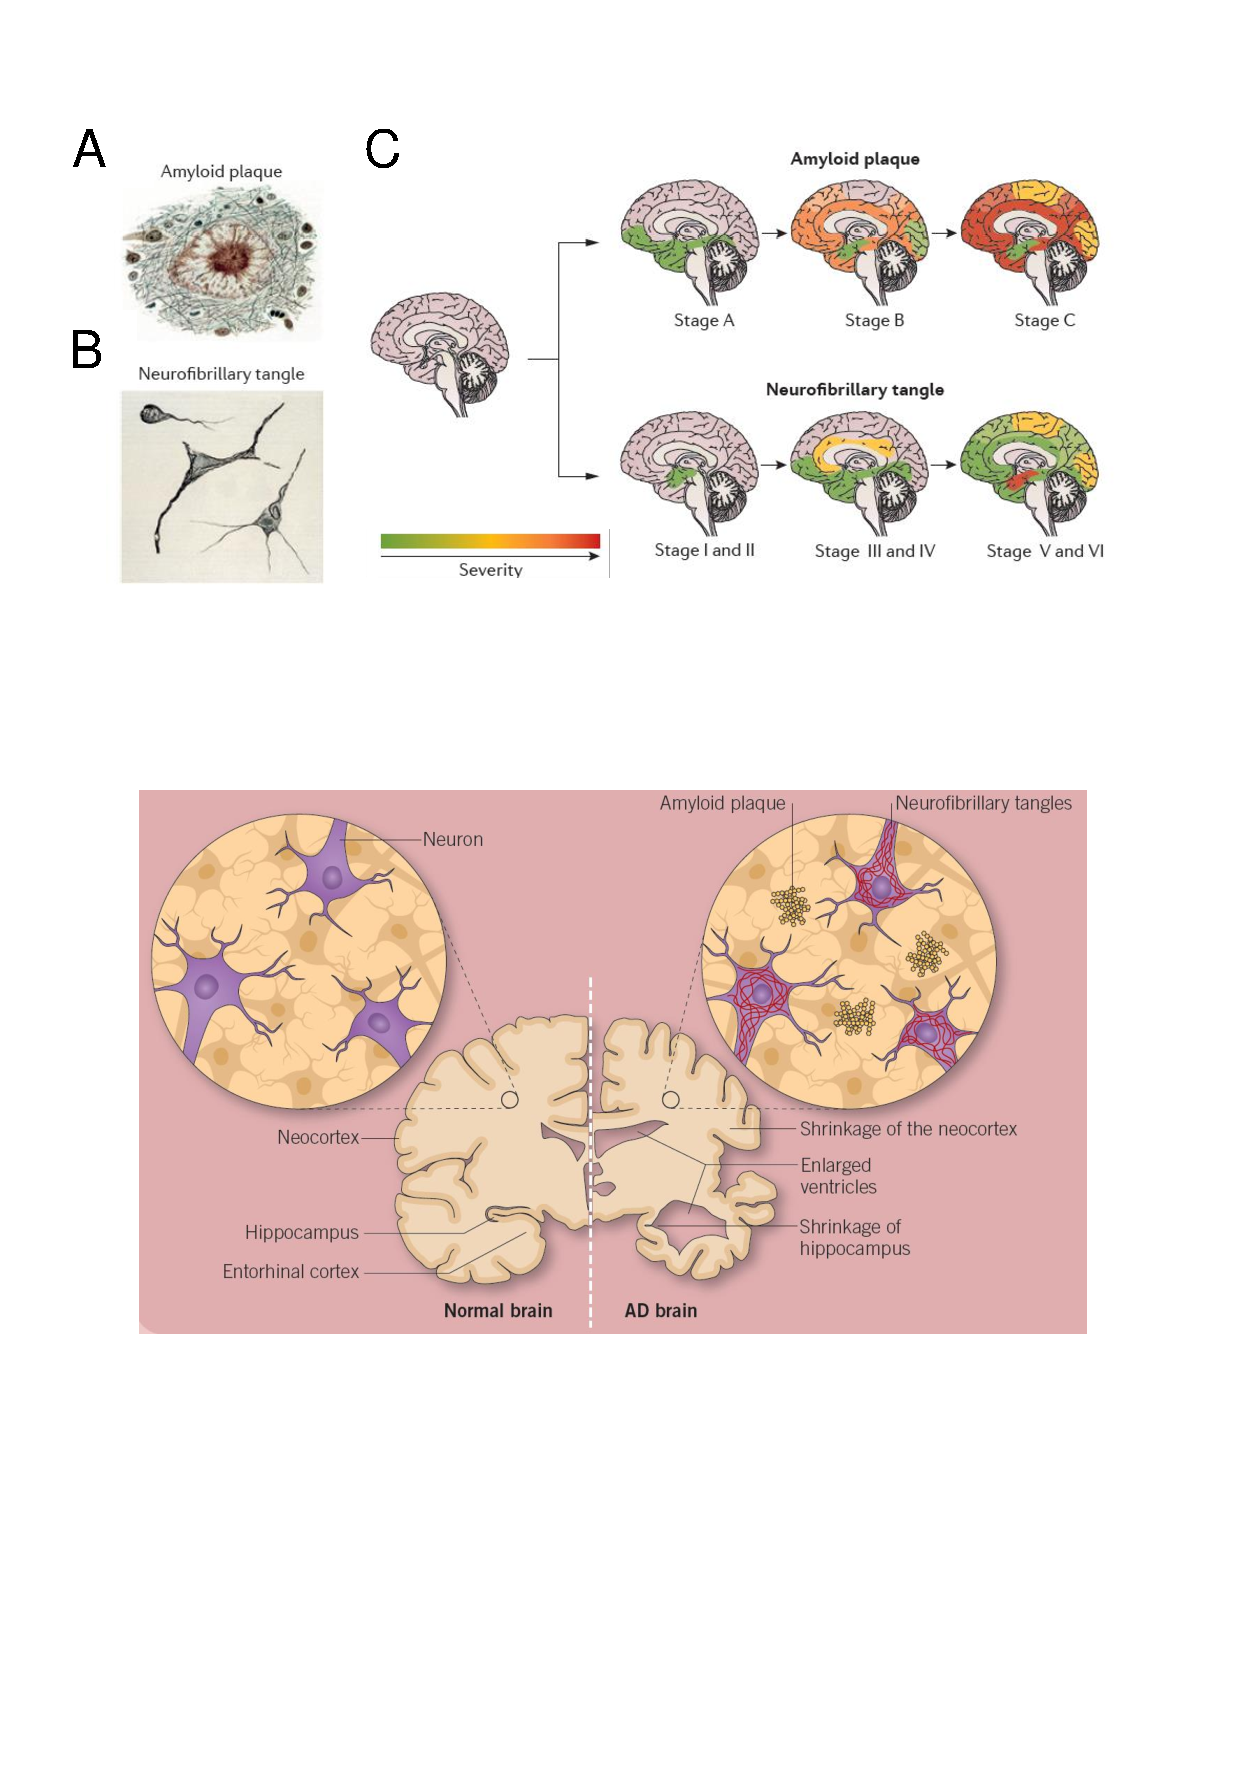
\includegraphics[page=1,trim={0 7cm 1cm 12cm},clip, scale = 0.8]{Figures/Introduction_Figures.pdf}
	\captionsetup{width=0.95\textwidth,singlelinecheck=off}
	\caption[Two key hallmarks of AD Neuropathology: amyloid plaques and neurofibrillary tangles]%
	{\textbf{Two key hallmarks of AD Neuropathology: amyloid plaques and neurofibrillary tangles}: Schema comparing a normal healthy brain and a brain with advanced AD. AD pathology is well characterised by the presence of extracellular amyloid plaques and intracellular neurofibrillary tangles, accompanied by significant neuronal loss and subsequent shrinkage of the neocortex and hippocampus. Figure is taken from Palmer (2015)\cite{AlanM.Palmer2015}
	}
	\label{fig:AD_intro}
\end{figure} 

\begin{figure}[!htp]
	\centering
	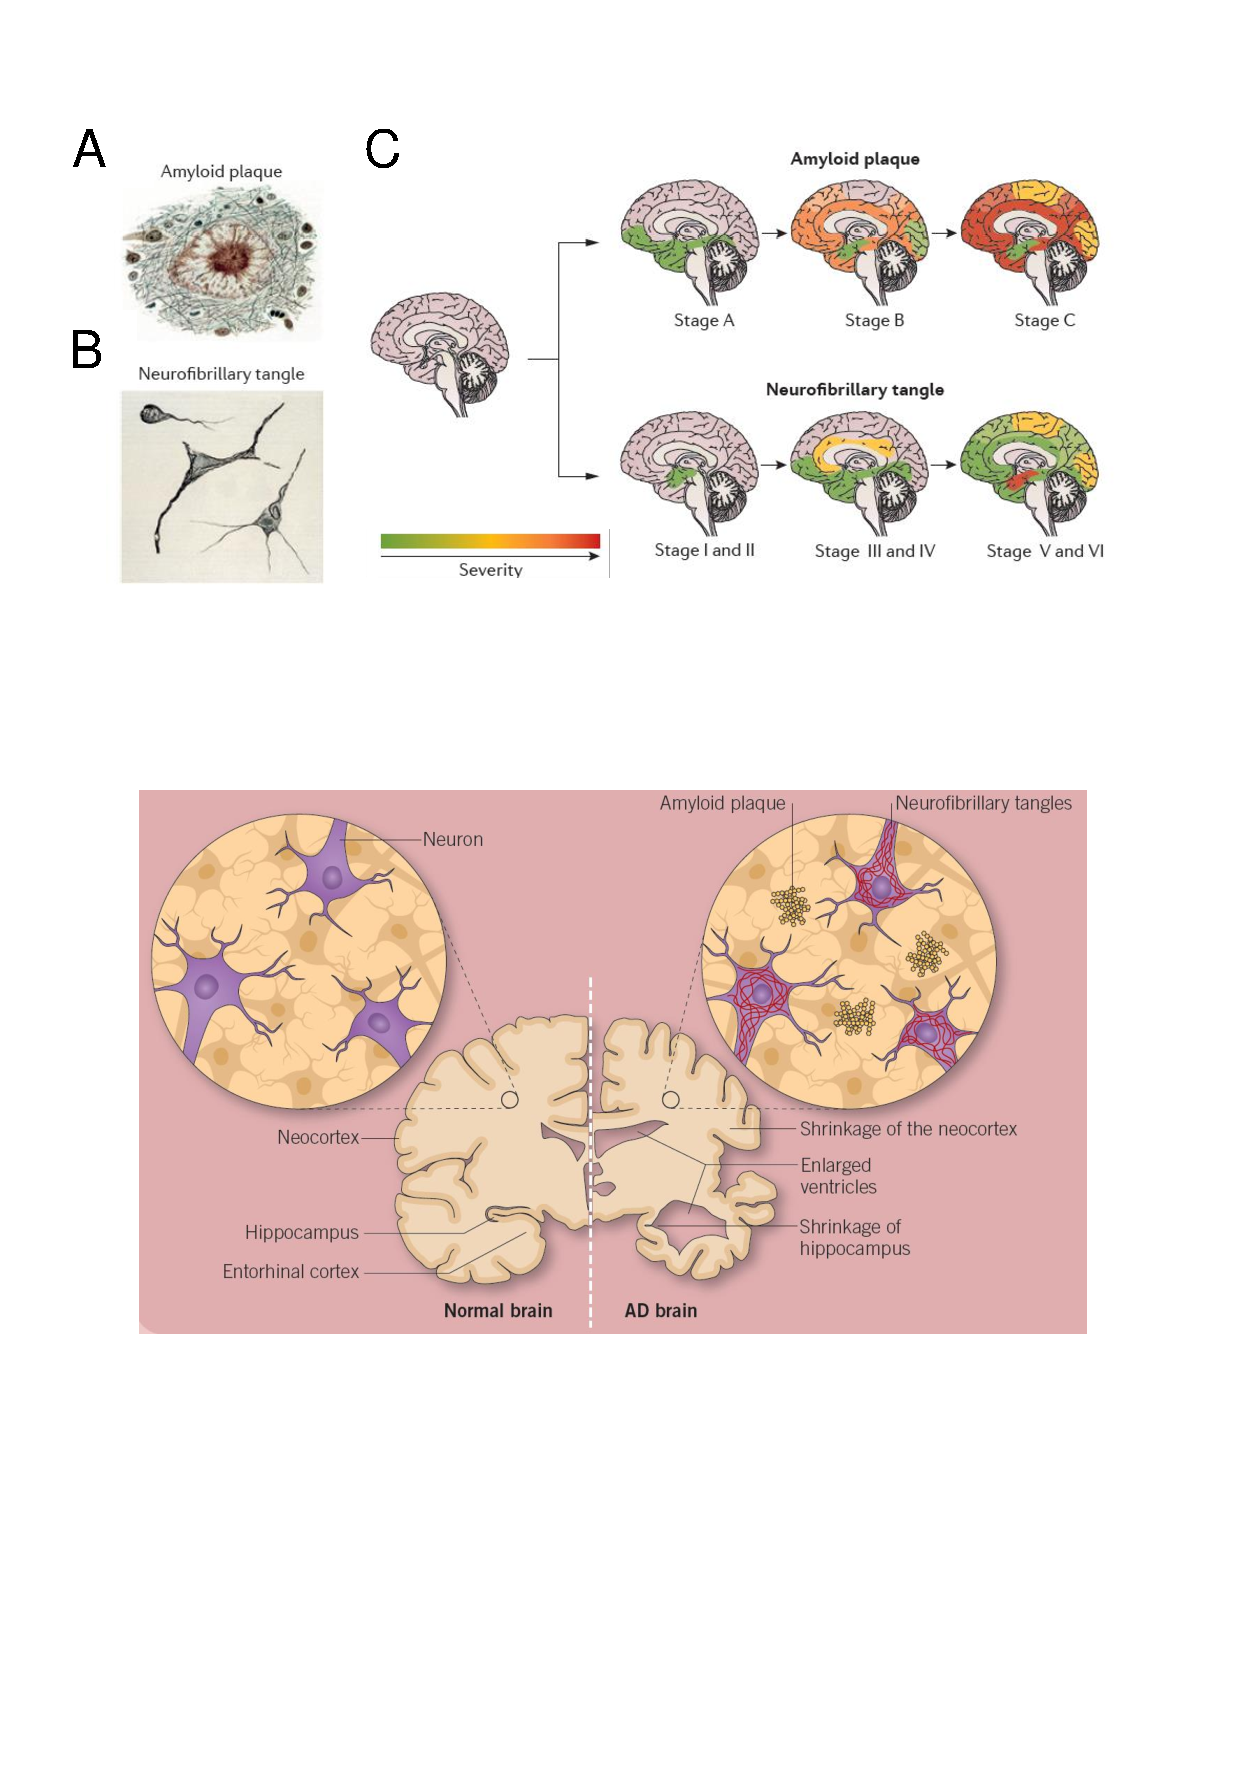
\includegraphics[page=1,trim={0 19cm 0cm 0cm},clip, scale = 0.8]{Figures/Introduction_Figures.pdf}
	\captionsetup{width=0.95\textwidth,singlelinecheck=off}
	\caption[Progression of amyloid plaques and neurofibrillary tangles with AD development]%
	{\textbf{Progression of amyloid plaques and neurofibrillary tangles with AD development}: Progression of \textbf{a)} amyloid plaques consisting of A$\beta$ measured according to Thal Phasing\cite{DR2002}, and \textbf{b)} neurofibrillary tangles composed of hyper-phosphorylated tau by Braak staging\cite{H1991}. Figure is taken from Masters et al.(2015)\cite{Masters2015}. 
		\\
		\\ 
		The deposition of A$\beta$ (Figure a) can be mapped Thal Phasing from a) the neocortex, to b) allocortical regions comprising of the entorhinal cortex and hippocampus, the striatum, and finally to iv) subcortical regions\cite{DR2002}. 
		\\
		\\
		In a similar pattern, the progressive spread of NFTs can be classified under the six stages of Braak (Figure b) from i,ii) the transentorhinal regions such as the entorhinal cortex, to the iii) hippocampus, iv) adjoining neocortex and finally to vi,v) other neocortical regions\cite{H1991}. 	
	}
	\label{fig:AD_development}
\end{figure}

\subsection{The genetics of Alzheimer's disease}
Although AD predominantly affects people aged 65 and above (referred as Late-Onset Alzheimer’s disease, LOAD\nomenclature{LOAD}{Late Onset Alzheimer's Disease}), 5\% of AD cases arise in much younger patients (Early-Onset Alzheimer’s disease, EOAD\nomenclature{EOAD}{Early Onset Alzheimer's Disease}). EOAD is normally associated with a clear familial autosomal dominant pattern of inheritance (Familial Alzheimer’s disease, FAD\nomenclature{FAD}{Familial's Alzheimer's Disease})\cite{Jarmolowicz2015}. To date, more than 160 highly-penetrant, causative mutation have been identified in EOAD, all located within three genes involved in amyloid plaque formation: \textit{APP} (amyloid precursor protein\nomenclature{APP}{Amyloid Precursor Protein}), \textit{PSEN1} and \textit{PSEN2} (presenilin 1 and 2\nomenclature{PSEN1}{Presenilin 1}\nomenclature{PSEN2}{Presenilin 2}) \cite{LM2010,Chai2007}. %While the clinical manifestations and presentation of neurological hallmarks are similar between EOAD and LOAD, patients with EOAD performed significantly worse in cognitive abilities not involved with memory (such as executive functions, language and visuoconstructional abilities)\cite{Joubert2016}.

While LOAD does not follow a Mendelian inheritance pattern, a relatively high heritability rate of 50-80\% \cite{Gatz2006} has been reported, indicating that there is still a large genetic predisposition for developing AD in later years. Indeed over recent years, genome-wide association studies (GWAS\nomenclature{GWAS}{Genome-wide association studies}) and subsequent meta-analyses \cite{Bellenguez2020,Naj2020,Kunkle2019,Jansen2019,Lambert2013,Naj2011,Hollingworth2011,Harold2009,Lambert2009,Bertram2008} have identified over 75 genetic loci associated with an increased risk of developing LOAD. These GWAS loci are typically changes (or variants) at a single DNA base-pair (single-nucleotide polymorphisms – SNPs\nomenclature{SNP}{Single Nucleotide Polymorphism}) that are found at a higher frequency in individuals with LOAD than in individuals without AD. 

The strongest genetic risk factor identified for LOAD to date is the $\epsilon$4 allele of \textit{APOE}\cite{Lambert2013}, the gene encoding for the cholesterol transporter apolipoprotein E (ApoE). This protein is a key regulator of lipid homeostasis, mediating lipid transport between astrocytes and neurons, a process critical for synaptic function and maintenance\cite{DH2001}. Harbouring one APOE$\epsilon$4 allele increases the risk of developing LOAD by 3-4x, while harbouring two $\epsilon$4 alleles increases the risk by 15x \cite{Farrer1997}; conversely, the $\epsilon$2 allele is known to confer a neuroprotective effect against AD \cite{Nagy1995,EH1994}. Although the $\epsilon$4 allele is estimated to occur in \textasciitilde 15\% of the general population, it has been observed in 40\% of patients with LOAD\cite{Farrer1997}. 

With the exception of \textit{APOE}, all the other genetics variants identified in GWAS are either common but lowly penetrant (such as those annotated to \textit{CLU, PICALM, CR1}) or highly penetrant but rare (e.g. those annotated to \textit{TREM2}) and collectively only contribute modestly to the risk of developing AD, highlighting the polygenic nature of AD (\cref{fig:AD_gwas}). While the molecular mechanisms through which these variants increase risk currently remains poorly understood, many are annotated to genes enriched in specific biological pathways, such as endocytosis, the immune system and inflammatory response, and lipid metabolism (described in \cref{aetiologyAD}). 


\begin{landscape}
	\begin{figure}[!htp]
		\centering
		\includegraphics[page=11,trim={0 17cm 0cm 1cm},clip, scale = 1.2]{Figures/Introduction_Figures.pdf}
		\captionsetup{width=1.6\textwidth,singlelinecheck=off}
		\caption[Genetic landscape of AD]%
		{\textbf{Genetic landscape of AD}: Shown are the genes implicated in AD from the causative EOAD genes (\textit{APP, PSEN1, PSEN2}) identified from early family studies, to the genes identified from GWAS studies annotated with either common but lowly penetrant or highly penetrant but rare variants. Variant penetrants, or effect size, is measured with the odds ratio (OR) with a larger odds ratio referring to a larger effect size. Variants conferring a protective effect are denoted in orange, and those with a negative effect in blue. Figure was taken from DeRojas et al. (2021)\cite{DeRojas2021}. GWAS - Genome-Wide Association Study, OR - odds ratio
		}
		\label{fig:AD_gwas}
	\end{figure}
\end{landscape}

\subsection{Molecular Mechanisms underpinning AD}
\label{aetiologyAD}
Despite the fact that AD neuropathology has been well described, the exact biological mechanisms driving AD onset and pathogenesis are still widely unknown. To date, there are two key hypotheses proposed for the progression of AD: i) the amyloid cascade hypothesis, ii) the tau tangle hypothesis. Results from GWAS, however, implicate other pathways that could be involved including a dysfunctional immune response, lipid metabolism, endocytosis, and cell-adhesion molecule (CAM) pathways for synaptic signalling.  

\boldheader{Amyloid cascade hypothesis} 
The amyloid cascade hypothesis posits that the extracellular accumulation of A$\beta$ is the key driver of AD pathogenesis, which initiates a pathological cascade of NFT, cell loss, vascular damage \cite{Hardy1992}. A$\beta$ is comprised of short peptides (39-43 amino acids) \cite{J1987} produced from the amyloidogenic cleavage of APP (a transmembrane protein involved in synapse formation and stability) by $\beta$-secretase (BACE - β-site APP-cleaving enzyme 1\nomenclature{BACE}{Beta-secretase}) and $\gamma$-secretase (a complex protein consisting of PSEN1 and PSEN2) (\cref{fig:APP_Processing}). Due to cleavage at various sites, $\gamma$-secretase produces A$\beta$ of varying lengths, with 90\% secreted as A$\beta$\textsubscript{40} and the remaining 10\% as A$\beta$\textsubscript{42}\cite{Asami-Odaka1995}.

\vspace{1cm}
\begin{figure}[!htp]
	\centering
	\includegraphics[page=2,trim={0 9cm 0cm 15cm},clip, scale = 0.8]{Figures/Introduction_Figures.pdf}
	\captionsetup{width=0.95\textwidth,singlelinecheck=off}
	\caption[Sequential cleavage of APP into A$\beta$ by $\beta$-secretase and $\gamma$ secretase]%
	{\textbf{Sequential cleavage of APP into A$\beta$ by $\beta$-secretase and $\gamma$ secretase}: Schema depicting sequential cleavage of APP, a transmembrane protein, either through the \textbf{a)} non-amyloidogenic pathway or \textbf{b)} the amyloidogenic pathway.
		\\
		\\
		In the non-amyloidogenic pathway, APP is cleaved by ADAM protein family (primarily, ADAM10, also known as $\alpha$-secretases) followed by $\beta$-secretase. Conversely in the amyloidogenic pathway, APP is sequentially cleaved by by $\beta$-secretase and $\gamma$-secretase, which can produce A$\beta$ of varying lengths. Monomeric A$\beta$ molecules, particularly, A$\beta$42, have increased propensity to oligomerise and aggregate to form the fibrils and plaques that are characteristic of AD. Figure is taken from Acker et. al (2019)\cite{Acker2019}. 
	}
	\label{fig:APP_Processing}
\end{figure}

In AD, the processing of APP is altered with the vast majority of causative \textit{APP}, \textit{PSEN1} and \textit{PSEN2} mutations favouring the production of the longer and more self-aggregating A$\beta$42 \cite{Li2019,D1996,JT1993}, thereby promoting the formation of insoluble fibrils and plaques\cite{JT1993}. 

%https://www.nature.com/articles/nrn2620

%Although interestingly, the neuroprotective ApoE$\epsilon$2 allele while associated with intact cognition is also associated with AD pathology in the oldest old population\cite{DJ2009}, suggesting that an A$\beta$-independent mechanism may be at play.   

%"TREM2 mediated phagocytosis is critical for Aβ and neuronal debris clearance in AD (Kleinberger et al., 2014; Xiang et al., 2016; Yeh et al., 2016). Specifically, TREM2 expression is important for microglia to physically associate with Aβ plaques (Ulrich et al., 2014; Wang et al., 2016; Yuan et al., 2016; Jay et al., 2015, 2017a,b)." 

%"CD33 is elevated in the AD brain in microglia and infiltrating macrophages and is thought to modulate microglial activation and Aβ clearance (Griciuc et al., 2013; Walker et al., 2015).  In fact, knock-out of CD33 in AD mouse models results in reduced Aβ plaque burden (Griciuc et al., 2013). 

\boldheader{Tau tangle hypothesis} 
%https://pubmed.ncbi.nlm.nih.gov/33848474/
The tau hypothesis posits that the phosphorylation and aggregation of tau to form NFTs are the primary drivers of AD\cite{KS1986}, which is also the defining feature of more than 20 other neurodegenerative disorders known collectively as tauopathies\cite{Orr2017}. Tau, encoded by the \textit{MAPT} gene, is a microtubule-associated protein involved in microtubule maintenance and stability. 

Recent studies suggests that hyper-phosphorylated tau dissociates from microtubules and aggregates into filaments\cite{Grundke-Iqbal1986,Grundke-Iqbal1986a} (components of NFTs) that disrupt axonal transport and signal transmission, ultimately resulting in synpatic degeneration and loss\cite{Coomans2021} (\cref{fig:tau_hypothesis}).  Tau mutations associated with frontotemporal dementia and Parkinsonism (FTDP) \nomenclature{FTDP}{Frontotemporal dementia and parkinsonism} are found to induce conformational changes that increase the affinity for phosphorylation\cite{Alonso2004}. While no causative mutations in \textit{MAPT} have been identified in AD, the severity of NFTs has shown to correlate better with cognitive decline and disease progression than amyloid plaques \cite{Serrano-Pozo2016,Giannakopoulos2003,PV1992} with its spread traced through Braak staging \cite{H1991} (\cref{fig:AD_development}\textbf{b}).

%Regional variation in MAPT mRNA and protein expression was observed with a 2-fold higher level in the neocortex than the cerebellum, any may explain regional vulnerability of brain regions to tau pathology\cite{Trabzuni2012}. 

\boldheader{Endocytosis} 
Endocytic processing (i.e. the internalisation of substrates into the cell) is directly implicated in AD due to distinct cellular localisation of secretases involved in the amyloidogenic processing of APP\cite{Acker2019}. Contrary to the non-amyloidogenic pathway that predominantly occurs at the plasma membrane\cite{Sisodia1992}, amyloidogenic processing of APP takes place in the endosome and is spatially regulated: BACE1 and PSEN1/$\gamma$ complex are localised at the plasma membrane and thus must first undergo endocytosis before assemblage with PSEN2/$\gamma$ secretase at the endosome (\cref{fig:APP_Trafficking}). Increasing evidence suggest that regulation of this endocytic pathway is altered in AD, creating an intracellular pool of A$\beta$ peptides \cite{Peric2015}; pathological significance of these intraneuronal peptides have been corroborated in AD mouse models with their appearance coinciding with cognitive deterioration in AD mouse models \cite{Tomiyama2010,Knobloch2007,Billings2005} and with stronger association to neuronal loss than A$\beta$ plaques\cite{Christensen2008}. Indeed, several risk genes emerging from recent GWAS are directly involved in endocytic regulation of APP processing, including: i) \textit{Bin1}, ii) \textit{Picalm}, and iii) \textit{Sorl1}, which encodes for SORLA (encoded by \textit{SORL1}), an APP-binding receptor involved in APP trafficking away from the late endosome for amyloidogenic processing and facilitating A$\beta$ degradation in lysosome \cite{Schmidt2016,Dumanis2015}.   

\vspace{1cm}
\begin{figure}[!ht]
	\centering
	\includegraphics[page=13,trim={0 14cm 0cm 2cm},clip, scale = 0.7]{Figures/Introduction_Figures.pdf}
	\captionsetup{width=0.95\textwidth,singlelinecheck=off}
	\caption[Tau hypothesis in AD]%
	{\textbf{Tau dissociation from microtubules and aggregation into NFTs}: Schema depicting a \textbf{a)} healthy and \textbf{b)} diseased neuron, with hyper-phosphorylated tau (orange spikes) detaching from microtubules. This results in microtubule dissociation and subsequent interrupted neuronal growth and function, essential for synaptic transmission. Figure is taken from Brunden et al. (2009)\cite{Brunden2009}
	}
	\label{fig:tau_hypothesis}
\end{figure}	


\begin{figure}[!htp]
	\centering
	\includegraphics[page=6,trim={0 8cm 0cm 0cm},clip, scale = 0.8]{Figures/Introduction_Figures.pdf}
	\captionsetup{width=0.95\textwidth,singlelinecheck=off}
	\caption[Spatial regulation of APP trafficking and processing]%
	{\textbf{Spatial regulation of APP processing}: Schema depicting APP trafficking and processing through the non-amyloidogenic (\cref{fig:APP_Processing}\textbf{a}), which predominantly occurs at the plasma membrane (boxed green), and amyloidogenic pathway (\cref{fig:APP_Processing}\textbf{b}), which preferentially occurs in the endosome (boxed red). APP processing through the amyloidogenic pathway is spatially regulated by the localisation and distinct internalisation of assembled PSEN1/$\gamma$ complex and BACE1 at the plasma membrane (boxed purple) and PSEN2/$\gamma$ in the endosome. Figure is adapted from Acker et. al (2019)\cite{Acker2019}  
	}
	\label{fig:APP_Trafficking}
\end{figure}



\boldheader{Immune Response}
Profound neuroinflammation, an inflammatory response within the CNS primarily orchestrated by the activation of microglia (microgliosis) and astrocytes (astrogliosis) with heightened release of cytokines, has been widely implicated in AD development pathology \cite{Cisbani2021,Griciuc2021}. While the role of the immune response is poorly understood in AD, it is widely accepted that an imbalance of the innate immune response is at play\cite{Frost2019} (\cref{fig:microglia_AD}\textbf{a}). Reactive microglia has been found surrounding amyloid plaques\cite{PL1987}, suggesting that plaque-associated microglia have a compromised phagocytic ability to remove A$\beta$\cite{Mawuenyega2010} - a complex process that involves recognition of toxic species (in this case, detrimental protein aggregates) by receptors, such as TREM2, CD33 and CR1, which are all GWAS AD risk genes. (\cref{fig:microglia_AD}\textbf{b}). Furthermore, reactive microglia can also release pro-inflammatory neurotoxic cytokines that can trigger neuronal apoptosis\cite{Qin2002,Wang2015b} and upregulate β-secretase\cite{Chen2012}, resulting in enhanced A$\beta$ propagation (\cref{fig:microglia_AD}\textbf{b}).  

Multiple recent transcriptomic profiling studies of single cells in AD human post-mortem brain tissue\cite{Mathys2019,Nott2019,Thrupp2020,Olah2020,Leng2021,Young2021} and AD mouse models\cite{Keren-Shaul2017,Mathys2017} have revealed subpopulations of microglia and astrocytes that have an altered molecular expression signature associated with disease progression. Proliferation of these distinct AD-associated microglial cells were accompanied with release of pro-inflammatory cytokines and increased expression of interferon-response genes\cite{Mathys2017}. Similar microglial cell states (termed disease-associated microglia - DAM\cite{Keren-Shaul2017}, and activated response microglia - ARM\cite{Frigerio2019}) have been also characterised in mouse models with upregulated expression in innate immune response and interferon pathways. Moreover, these AD-associated microglia subpopulations were enriched with altered expressions of \textit{Trem2} and \textit{Cd33} \cite{Mathys2019,Frigerio2019}. A subset of AD-associated astrocytes, likely to represent reactive astrocytes, has also been characterised with upregulated expression of \textit{Gfap} and \textit{Cd44}, and downregulation of genes associated with homeostasis\cite{Leng2021}. Notably, the largest proteomic study to date identified that the protein co-expression module most robustly associated with AD and FTD was also associated in astrocyte- and microglial-associated proteins, and was significantly enriched in AD GWAS genes and protective markers of anti-inflammatory disease-associated microglia \cite{Johnson2020}.    

%Role of adaptive immune response with recent identification of a subpopulation of immune cells, CD8+ T effector memory CD45RA+ (TEMRA), associated with AD pathology and exhibited stronger antigenic stimulation (increase in cytokine signalling) \cite{Gate2020}. In addition to the stronger-associated AD risk variants, previous studies have identified additional rare coding variants in genes involved in the immune response\cite{R2017,Bis2018} and transcriptional regulation\cite{Bis2018}.

\begin{figure}[!htp]
	\centering
	\includegraphics[page=8,trim={0 8cm 0cm 0cm},clip, scale = 0.8]{Figures/Introduction_Figures.pdf}
	\captionsetup{width=0.95\textwidth,singlelinecheck=off}
	\caption[Role of microglia in AD development and pathology]%
	{\textbf{Role of microglia in AD development and pathology}: A simplified schema illustrating the \textbf{a)} multifaceted roles of microglia in AD, ranging from a protective to a detrimental role by the respective secretion of anti- and pro-inflammatory cytokines, and \textbf{b)} Microglia's dual response to A$\beta$ plaques, either through A$\beta$ clearance or release of pro-inflammatory cytokines. Recent emergence of single RNA-sequencing studies have revealed significant heterogeneity in microglia isolated from AD post-mortem brain tissues, highlighting the complex role that microglia plays in AD development and pathology. Under physiological conditions, the microglia is ramified. PRR - Pattern recognition receptors, such as TREM2 and CD33, are found on the cell surface of microglia and are involved in recognising toxic species for phagocytosis. Both figures are adapted from Leng et al. (2021)\cite{Leng2021a}  
	}
	\label{fig:microglia_AD}
\end{figure}


\boldheader{Lipid Metabolism}
\label{intro_lipid}
Identification of \textit{Apoe} $\epsilon$4 variant as the most robustly LOAD-associated genetic variant established a link between lipid metabolism and AD. Increasing evidence further postulates that A$\beta$ clearance is regulated in an APOE isoform-dependent manner\cite{Castellano2011} with APOE4 having low binding affinity to A$\beta$ and thus, being the least efficient at A$\beta$ clearance\cite{RM2012} - carriers of $\epsilon$4 allele have more pervasive amyloid plaques than non-carriers\cite{DE1993,E2009}. APOE lipidation status, mediated by ABCA1\cite{R2010}, has also been reported to impact A$\beta$ aggregation, with APOE4 being poorly lipidated compared to APOE2 and APOE3, resulting in increased propensity to aggregate\cite{DM2006}. 

More broadly, lipid metabolism and homeostasis are linked to AD development in that APP, $\beta$- and $\gamma$-secretase are transmembrane proteins (\cref{fig:APP_Trafficking}); lipid membrane constitution and organisation would therefore have an impact on the APP trafficking and secretase activities \cite{DiPaolo2011}. \textit{ABCA7}, by regulating the lipid composition at bilayer, can indirectly influence the activity and expression of $\beta$-secretase \cite{Sierksma2020,Sakae2016}.  

%CLU

\boldheader{Interplay of multiple molecular pathways}
While the two key hypothesis of amyloid plaque formation and tau aggregation are widely supported, identification of AD-associated genes, enriched in multiple pathways, highlight the complexity and multifacetted nature of the disease. As described above, genetic studies of AD strongly implicate pathways centred on abnormal A$\beta$ trafficking, processing, and clearance. Recent studies have also revealed interplay between pathways, with APOE4-expressing microglia exhibiting less active transcriptional response and reduced uptake A$\beta$ than APOE3-expressing microglia, which is further exacerbated by Trem2 deficiency\cite{Fitz2021}.  


%https://science.sciencemag.org/content/370/6512/61?rss=1


%\boldheader{Synpatic signalling} 

\clearpage
\subsection{Modelling AD: Transgenic Mouse Models}
While profiling human post-mortem brain tissues remains the gold standard for studying AD pathogenesis, there are various confounding secondary factors (e.g. environmental exposures such as diet, medication) and technical difficulties (e.g. agonal state and post-mortem interval impacting RNA quality) to consider. In comparison, mouse models of disease can be tightly controlled (i.e. for genotype, living conditions, their age and pathological status) to enable analyses into the progression of pathology in disease-relevant cell-types.  

To study the different aspects of pathology, a number of transgenic AD mouse models have been developed with mutations that either result in amyloidopathy (formation of A$\beta$ plaques) or tauopathy (NFT) (\cref{tab:mouse_models}). Amyloidopathy is typically developed through the insertion and overexpression of human \textit{APP}, either alone or in combination with \textit{PSEN1}, whereas tauopathy is recapitulated by overexpressing human \textit{MAPT} with FTD-associated mutations (given no causative \textit{MAPT} mutations have been identified in AD). The insertion of transgenes, however, have been found to disrupt endogenous mouse genes that may significantly contribute to the neurodegenerative phenotype observed in these mice. 

It is also important to note that there are currently no mouse model that encapsulates all the defining features of AD and one of the major criticisms of current AD mouse models relates to how representative they are of sporadic, late-onset AD. There have been recent efforts to generate mouse models that more closely resemble LOAD with the incorporation of AD-associated variants, such as $\epsilon$ variant of \textit{APOE} and R47H \textit{Trem2} variant \cite{apoe4trem2_mousemodel,Lewandowski2020}, however these are not widely used.

Nonetheless, current mouse models act as a valuable reductionist tool to dissect the processes that drive the onset and study the pathology of AD pathology, identify biomarkers and validate novel targets\cite{Hall2012}. In my thesis, I utilise the rTg4510 mouse model to profile progressive changes in splicing and isoform regulation associated with development of tau pathology. More details about this model are provided in \cref{ch: general methodology}. 


\begin{table}[htp]
	\centering
	\setlength\tabcolsep{3.5pt}
	\captionsetup{width=1\textwidth}
	\caption[Representative AD Mouse Models]%
	{\textbf{Representative AD mouse models}. Tabulated is a list of the most widely used AD mouse models developed from overexpression of one or more genes associated with FAD. Table is adapted from Hall et al. (2012) \cite{Hall2012} and is by no means comprehensive. mo - months}
	\label{tab:mouse_models}
	\begin{threeparttable}
		\begin{tabular}{@{}lllcccc@{}}
			\toprule
			\multicolumn{2}{c}{Mouse Models} &
			\multicolumn{1}{c}{Mutations} &
			\begin{tabular}[c]{@{}c@{}}Plaques\\  (mo)\end{tabular} &
			\begin{tabular}[c]{@{}c@{}}Tangles\\   (mo)\end{tabular} &
			\begin{tabular}[c]{@{}c@{}}Neuronal \\ Loss (mo)\end{tabular} &
			\begin{tabular}[c]{@{}c@{}}Cognitive \\ Deficit (mo)\end{tabular} \\ \midrule
			\multirow{4}{*}{hAPP}     & PDAPP                 & Ind\tnote{b}                        & 6  & x  & x     & 6                \\
			& Tg2576                & Swe\tnote{a}             & 11 & x  & x     & \textgreater{}12 \\
			& J20                   & Swe\tnote{a}, Ind\tnote{b} & 6  & x  & x     & 4                \\
			& APP23                 & Swe\tnote{a}               & 6  & x  & 14-18 & 3                \\
			\multirow{3}{*}{hAPP/PS1} & PS/APP & Swe\tnote{a}, M146L\tnote{e}                 & 6  & x  & 22    & 3                \\
			& APP/PS1         & Swe\tnote{a}, PSEN1dE9              & 6  & x  & x     & 6                \\
			& 5xFAD                 & Swe\tnote{a}, Lon\tnote{a}, Flo\tnote{c}, M146L\tnote{e}, L28V\tnote{e} & 2  & x  & 9     & 4                \\
			\multirow{4}{*}{hTau}     & hTau.P301S            & MAPT P301S                 & x  & 4  & 3     & 3                \\
			& 3xTg                  & Swe\tnote{a}, MAPT P301L, M146V     & 6  & 12 & -    & 4                \\
			& rTg4510               & MAPT P301L                 & x  & 4  & 6     & 3                \\
			& htau                  & Wildtype                   & x  & 9  & 10    & 6                \\ \cmidrule(l){1-7} 
		\end{tabular}
		\begin{tablenotes}
			\footnotesize
			\item[a] Swedish APP mutation K670N/M671L
			\item[b] Indiana APP mutation V717F
			\item[c] London APP mutation V717I
			\item[d] Florida APP mutation I716V 
			\item[e] Human PSEN1 mutations 
		\end{tablenotes}
	\end{threeparttable}
\end{table}


%rtg4510: https://journals.plos.org/plosone/article?id=10.1371/journal.pone.0106050


\clearpage
\section{Transciptional dysregulation in AD}

The vast majority of variants associated with LOAD are annotated to non-coding regulatory regions of the genome, being enriched in open chromatin regions that promote transcription such as enhancers\cite{Kikuchi2019} (short DNA sequences containing specific motifs for binding of transcription factors). Recent single cell studies have further demonstrated that AD-associated non-coding SNPs are enriched in microglia enhancers with cell-type specific regulation of gene expression\cite{Tansey2018,Nott2019,Young2021,Novikova2021}, suggesting that AD-associated risk variants mediate disease associations through gene regulation. 

Efforts to better understand the expression changes in AD by profiling the complete set of expressed RNA transcripts (hereby referred as transcriptome) in AD mouse models and post-mortem brain tissues have been essential in revealing insights into the molecular mechanisms that underlie AD risk variants. A number of studies have identified widespread gene differences in transgenic mice harbouring AD-associated mutations and affected post-mortem brain regions (reviewed in XXX). Recent works in our group have similarly identified robust changes in gene expression associated with tau pathology development in rTg4510, with these genes found to be enriched in pathways previously implicated in AD pathology\cite{Castanho2020}. In addition to expression changes observed at the gene level, there is increasing evidence for the role of altered splicing regulation (more detail is provided in \cref{intro:AD_alteredsplicing}). These AD-associated splicing changes are also enriched in genes involved in pathways previously implicated such as the immune response and synaptic transmission, adding to the layer of complexity underlying AD pathogenesis. 

%lead variant of \textit{BIN1} (rs6733839C>T) was preferentially located in OCR of microglia and predicted to increase binding affinity for MEF2C transcription factor, subsequently increasing \textit{BIN1} expression \cite{Young2021}. Deletion of microglia-specific enhancer reduced BIN1 expression in microglia, but not in neurons an astrocytes\cite{Nott2019}
%Transcriptomic landscape profiling of disease-relevant tissues, in taking a snapshot of the present state of the cells, is key to elucidating the functional relationship between the genetic variants identified from GWAS and the molecular mechanisms that drive disease development and pathology in a time- and tissue-dependent manner \cite{Verheijen2018}.  %https://pubmed.ncbi.nlm.nih.gov/31626773/
%Between all the regulatory mechanisms influencing gene expression, there is a growing recognition that non-coding variants effects are mediated through alternative splicing in neuropsychiatric diseases, including schzizophrenia and autism
%https://pubmed.ncbi.nlm.nih.gov/31451803/


\subsection{Alternative Splicing}
Alternative splicing is a transcriptional regulatory mechanism that produces distinct transcripts (isoforms) from a single gene, which are potentially translated to different protein isoforms with unique, and potentially, antagonistic functions\cite{Wang2008}. It is a widespread phenomenon with over 95\% of human genes estimated to be influenced \cite{Pan2008}, and is most prevalent in the brain\cite{Yeo2004}, where it impacts upon neuronal development and maintenance\cite{Pan2008, Mazin2014, Raj2015}. There is a growing recognition of the key role of aberrant mis-splicing in neurodegenerative diseases \cite{Gandal2018,RL2019}, including schizophrenia and autism. 

\boldheader{Mechanism}
Splicing involves the removal of non-coding sequences (introns) from mRNA precursors and the ligation of coding sequences (exons), resulting in isoforms with different exonic structures (\cref{fig:AS_events}). This relies on the concerted and regulated assembly of the spliceosome (a multimegaton, dynamic ribonucleoprotein complex) by its recognition and stepwise-binding to sequence elements within the pre-mRNA (cis-elements), and a group of regulating splicing factor proteins (trans-elements) (\cref{fig:AS_mechanism}). Recent studies suggest that this process occurs co-transcriptionally, such that the intron can be identified and removed as soon as it is synthesised by the RNA polymerase. 
%There are two types of spliceosome - major and minor - both of which involve the activity of five uridine-rich small nuclear ribonucleoproteins (snRNP\nomenclature{snRNPs}{Small Nuclear Ribonucleoproteins}) and numerous non-snRNP proteins\cite{Will2011}. Using a similar mechanism but composed of different snRNPs, the minor spliceosome removes less than 1\% (0.4\%) of introns\cite{Turunen2013} and is thus referred to as "U12-dependent non-canonical splicing", as opposed to "U2-dependent canonical splicing" with major spliceosome.

Correct splicing first requires recognition of short sequence motifs upstream (5' splice site, 5'SS\nomenclature{5'SS}{5' Splice Site}, donor site) and downstream (3' splice site, 3'SS\nomenclature{3'SS}{3' Splice Site}, acceptor site) of the intron/exon boundary, followed by sequential assembly of the spliceosome components and intron excision\cite{Herzel2017}. The 5'SS is typically defined by a conserved 9-nucleotide sequence with a GU(T) dinucleotide, and the 3'SS by a polypyrimidine tract (PPT\nomenclature{PPT}{Polypyrimidine Tract}) followed by a conserved AG dinucleotide \cite{Will2011}. Almost all introns in human and mouse are flanked by the GT-AG splice site dinucleotides\cite{Sheth2006} (termed splice junctions), with other dinucleotide variations known to exist in very minute proportions: GC-AG and AT-AC comprises \textasciitilde0.9 and \textasciitilde0.09\% of human splice sites\cite{Parada2014}. An increasing number of disease are linked to aberrant alternative splicing by pathogenic variants by interfering cis-acting elements (5'SS and 3'SS, resulting in exon skipping, exon inclusion, exon extension or exonic splice gain; intron resulting in intron gain) and action of trans-acting protein splicing factors.

%Alternative splicing is highly-regulated in a temporal and cell-specific manner by the binding and fin-tune balance of trans-acting factors to cis-acting elements. The sequence of these cis-acting elements within the exon (exonic splicing - ES) or intron (intronic splicing - IS) determines the binding affinity of the trans-acting factors to either enhance or suppress splicing. RNA structure also plays a role in blocking or allowing trans-acting factors to bind, and transcription factor assemblage through distal interactions. 
%Trans-acting factors include RNA-binding proteins such as SR protein (serine and arginine-rich proteins), heterogeneous nuclear ribonucleoproteins (hnRNPs, and other tissue-specific proteins and complementary microRNA (miRNAs); Cis-elements include exonic splicing enhancers and silencers ( ESEs, ESSs), intronic splicing enhancers and silencers (ISEs, ISSs). Localisation and function of trans-factors are further regulated by post-translational modifications, adding to the layer of complexity through activation/suppression from other proteins involves post-translational modifications i.e. kinases and phosphatases. 


\vspace{1cm}
\begin{figure}[!htp]
	\centering
	\includegraphics[page=9,trim={0 16.5cm 0cm 0},clip, scale = 0.7]{Figures/Introduction_Figures.pdf}
	\captionsetup{width=0.95\textwidth,singlelinecheck=off}
	\caption[Alternative Splicing Events]%
	{\textbf{Alternative Splicing Events}: Splicing involves removal of introns and ligation of exons either constitutively or alternatively to generate isoforms with different exonic structure: an exon can be entirely skipped (orange exon in SE) or two exons that are not spliced together (orange and blue exon in MX), an intronic sequence can be retained (light orange in IR), a different 5'SS or 3'SS can be used resulting in a novel splice junction (A5', A3'), and the usage of different first and last exons which can result in an alternative promoter and termination.  
	}
	\label{fig:AS_events}
\end{figure}


\begin{figure}[!htp]
	\centering
	\includegraphics[page=3,trim={0 14cm 8cm 2cm},clip, scale = 0.8]{Figures/Introduction_Figures.pdf}
	\captionsetup{width=0.95\textwidth,singlelinecheck=off}
	\caption[Splicing Mechanism: spliceosome assembly on nascent RNA]%
	{\textbf{Intron removal is catalysed by the assembly and complex rearrangement of spliceosome. a)}:  Consensus sequence of splice sites that demarcate the intron/exon boundary and are essential for recruitment of spliceosomal snRNPs. \textbf{b)} Co-transcriptional assembly of spliceosome with stepwise interaction of spliceosomal snRNPs, with the formation of 
		\begin{enumerate}
			\item E (Early) commitment complex with the identification and binding of U1 snRNP to the 5'SS and branchpoint binding protein (BPP\nomenclature{BPP}{Branchpoinnt Binding Protein} to BPS 
			\item A (Assembly) catalytically-active complex with association of U2 snRNP to the branch site following the dissociation of BPP. The "A" here denotes to the adenosine of BPS
			\item B pre-catalytic spliceosome complex with recruitment of U4,U5 and U6 snRNPs
			\item B pre-catalytic spliceosome complex after major conformational rearrangements within the spliceosome (RNA-protein and RNA-RNA interactions) followed by the release of U1 and U4 snRNP to expose the adenosine from BP to the 5'SS 
			\item B* catalytically-active complex with nucleophilic attack of adenosine on 5'SS (first step of transesterification) 
			\item C catalytically-active complex with further conformational changes in the U2 snRNA to C* complex, with nucleophilic attack of the 5'SS to 3'SS (second step of trans-esterification) 
			\item P (Post-spliceosome complex). The mRNA product is then released from remaining spliceosome (ILS), now bound to the intron lariat. The snRNPs can then disassociate and be recycled for next cycle of splicing.
			\\
		\end{enumerate} 
		Intron excision is primarily executed by two trans esterification reactions.	BPS - Branch point sequence, CTD - carboxyl-terminal domain, ILS - Intron lariat spliceosome, PAS - poly(A) site, SS - Splice site, TSS - Transcription start site,TTS - Transcription termination site. Figure is taken from Herzel et al. 2017\cite{Herzel2017}.
	}
	\label{fig:AS_mechanism}
\end{figure}

%\boldheader{Other regulatory mechanisms}
%Of note, splicing is only one of the main ways of gene regulation;pre-transcriptional regulation involving chemical modifications of DNA nucleotides (epigenetics), transcriptional regulation involving the binding of transcription factors and post-transcriptional regulation involving the processing of mRNA transcripts. Splicing works with these mechanisms together (?). 
%AS further regulates gene expression through various mechanisms: non-sense mediated decay, miRNA-mediated mRNA degradation, altered translational efficiency of isoforms. In contrast, alternative polyadenylation regulates RNA transportation, localization, stability, and translation by generating splice isoforms with different cleavage sites. Nonsense mediated decay (NMD) \nomenclature{NMD}{Nonsense Mediated Decay} products are alternatively spliced isoforms that are not translated into proteins, by containing an early stop codon. A premature termination-translation codon highly supportive of NMD is defined by a stop codon within at least 50-55 base pairs upstream of splice junctions.  up to 70\% containing multiple polyadenylation sites and 60\% with two or more promoters from alternative transcription start sites \cite{Carninci2006}. In addition to above five common categories, many other complex types, such as alternative position, i.e., alternative 3' and 5' site (Wang and Brendel, 2006), AS and transcriptional initiation (ASTI) (Nagasaki et al., 2006) alternative first exons (Chen et al., 2007), and composite patterns (Wang and Rio, 2018), can occur.
%Introduction of variable segments within otherwise identical mRNAs, with 80% of this variability observed within open reading frames (ORFs), subsequently contributing significantly to proteome diversity, and 20% falling within untranslated regions that regulates cis-binding effects. (G. S. Wang & Cooper, 2007) Subsequently, influencing mRNA stability, translation efficiency (including miRNA binding sites), and mRNA localisation. One-third of alternative splicing events introduce premature termination codons (PTCs), which cause mRNA degradation by nonsense-mediated decay (NMD) (Lewis, Green, & Brenner, 2003). Therefore, alternative splicing regulates temporal and spatial expression of functionally diverse isoforms, on–off regulation by NMD, or other post-transcriptional regulatory responses; also for cell identity, whereby number of tissue-specific isoforms highest in the brain. 
%Still high error rate accuracy of nanopore "The raw accuracy of nanopore 1D cDNA sequencing is ~85–87%36–38, although accuracy can change depending on iterations of the technology and library preparation methods37" \cite{Tang2020}

\newpage
\subsection{Altered splicing in AD}
\label{intro:AD_alteredsplicing}
Dysregulation of splicing can have significant functional consequences in driving or contributing to disease progression and susceptibility, by disrupting protein isoform function (loss-of-function or gain-of-function) or generating an imbalanced isoform ratio (i.e. a change in relative isoform expression). Studies on the role of alternative splicing in AD have largely focused on specific FAD genes, such as \textit{PSEN1, APP and MAPT}; e.g. a mutation in intron 4 of PSEN1 produces aberrantly-spliced truncated PSEN1 isoforms that were found to increase A$\beta$42 \textit{in vitro}\cite{DeJonghe1999}. Perhaps more well known is the altered splicing of MAPT whereby exclusion or inclusion of exon 10 (E10) generate isoforms with either 3 (3R tau, E10-) or 4 (4R tau, E10+) microtubule-binding repeat domains, with the latter having a greater interaction with microtubules. Over 50 tauopathy-associated intronic mutations were found clustered around the 5'splice site of exon 10 in favouring inclusion of exon 10 \cite{DSouza1999, Ghetti2015}, resulting in increased production of 4R tau and imbalanced 4R/3R ratio that contribute to tau aggregation \cite{Adams2010} - mimicking this imbalanced ratio in a tauopathy mouse model induced more seizures, and more phosphorylated,self-aggregating tau \cite{Schoch2016}.  
%tau-isoform mediated neurodegeneration   
% efforts to better understand gene expression changes in AD by sequencing transcriptome of affected brain regions


%(Trabzuni et al 2012)(Rockentein et al 1995)(Buee et al 2000)(Valenca et al. 2016) studies on AS

Notably, multiple spliceosomal components were found to co-aggregate with tau in post-mortem AD brain tissues\cite{Bai2013}, indicating that there is a global change in the core splicing machinery and consequent disruption of splicing in AD pathogenesis. More recently, transcriptomic profiling of AD post-mortem brain tissues\cite{Raj2018} revealed aberrant splicing as a hallmark of AD. Furthermore, the study identified that AD-associated splice variants (splicing quantitive trait loci - sQTL) were enriched in transcriptionally active regions with overlap of AD-associated epigenetic variants (DNA methylation - mQTL, histone acetylation - hQTL), and AD-associated SNP. 
%highlighting region-specific deterioration associated with AD\cite{Mills2013}
%Evidence of upregulated levels of intron-retained transcripts in AD vs control, including in genes previous implicated in AD (Bin1,Picalm)\cite{Li2021}

%Applications of these novel bioinformatic approaches to study alternative splicing in AD human post-mortem brains revealed over 2000 genes with differential transcript usage, including \textit{APP} and \textit{BIN1} \cite{Marques-Coelho2021}.

\begin{changemargin}{1.5cm}
	%\captionsetup{width=30cm}
	\begin{landscape}
		\small %smaller font
		\setlength\tabcolsep{2pt} %reduced margin size in table
		\renewcommand{\arraystretch}{1}
		\begin{longtable}[c]{p{3cm}p{4cm}p{3cm}p{16cm}}
			\caption[Transcriptomic and Proteomic Studies in AD]%		
			{\textbf{Transcriptomic and proteomic studies in AD human post-mortem brain tissues in revealing mis-splicing as a widespead hallmark of AD}. \textsuperscript{a}RNA-Seq data from ROSMAP dataset. AS - Alternative Splicing, NMD - Nonsense Mediated Decay, RBP - RNA binding protein, TSS - Transcription Start Site}
			\label{tab: AS_ADHuman_studies}\\
			
			\toprule
			\multicolumn{1}{c}{References} &
			\multicolumn{1}{c}{Samples and Tissue} &
			\multicolumn{1}{c}{Method} &
			\multicolumn{1}{c}{Key Findings} \\* \midrule
			\endfirsthead
			%
			\endhead
			%
			\bottomrule
			\endfoot
			%
			\endlastfoot
			%		
			\centering Twine et al. (2011)\cite{Twine2011} &
			\centering 3 AD, 33 Controls\newline Total, frontal \& temporal lobe &
			\centering RNA-Seq &
			\tabitem \textit{Apoe} downregulated in AD temporal lobe and 3 isoforms with different TSS detected. Differential isoform expression detected: ENST00000252486 and ENST00000446996 from TSSA were downregulated (3.09-fold) whereas ENST00000425718 from TSSB was upregulated (26.5-fold) \newline
			\tabitem \textit{Ank1} downregulated in AD total brain \\
			\hdashline[0.5pt/5pt]
			
			\centering Mills et al. (2013)\cite{Mills2013} &
			\centering 5 AD, 5 Controls \newline Parietal lobe &
			\centering RNA-Seq &
			\tabitem Differentially expressed genes enriched in lipid metabolism (\textit{ACOT1}, \textit{ACOT2} and  \textit{DBI/ACBP} upregulated, \textit{TECR} downregulated) \newline
			\tabitem Differential isoform expression observed in \textit{DBI/ACBP}; non-coding DBI-009 upregulated while protein-coding DBI-003 is downregulated. \\
			\hdashline[0.5pt/5pt]
			
			\centering Bai et al. \newline(2013)\cite{Bai2013} &
			\centering 18 AD, 17 Controls \newline Cortex &
			\centering Mass Spectrometry, RNA-Seq &
			\tabitem Extranuclear aggregation of 36 proteins, including spliceosomal components (U1 snRNP, U1-70K) \newline
			\tabitem Accumulation of unspliced RNA molecules in AD, with reduced splicing efficiency (increased ratio of pre- and mature RNA) in AD-associated genes (\textit{BACE1, BIN1, CLU, GFAP, PICALM, PSEN1, SORL1})  \\
			\hdashline[0.5pt/5pt]
			
			\centering  Lai et al. \newline(2014)\cite{Lai2014} &
			\centering 8 AD, 8 Controls\newline Superior Temporal Gyrus &
			\centering Microarray &
			\tabitem 22 genes identified with differential AS event (characterised by differential exon usage) \newline  \tabitem \textit{GNAL} transcript variant 5 downregulated in AD whereas transcript variant 1 showed no change \newline  \tabitem \textit{MAP4} transcript variant 3 downregulated in AD whereas transcript variant 1 was upregulated\\
			\hdashline[0.5pt/5pt]
			
			\centering Mills et al. (2014)\cite{Mills2014} &
			\centering 14 AD, 16 Controls \newline Superior Temporal Gyrus &
			\centering RT-qPCR &
			No difference in total \textit{APOE}, \textit{APOE-005}, or \textit{APOE-001} between AD superior temporal gyrus and controls, contrary to Twine et al. (2011)\cite{Twine2011} \\
			
			\centering Humphries et al.(2015)\cite{Humphries2015} &
			\centering 10 AD, 10 Controls, \newline Temporal lobe &
			\centering RNA-Seq &
			9 genes differentially expressed (\textit{ABCA7, CR1, MS4A14, MS46E, PTK2B}), 5 of which had differential splicing (\textit{ABCA7, TMEM259, EPHA1, MS4A6A, MS4A6E}) defined by overall exon distribution differences\\
			\hdashline[0.5pt/5pt]
			
			\centering Magistri et al.(2015)\cite{Magistri2015} &
			\centering 4 AD,4 Controls \newline Hippocampus &
			\centering RNA-Seq &
			\tabitem Downregulation of \textit{TAC1} and upregulation of \textit{SERPINE1} \newline 
			\tabitem Pathway analysis indicate dysregulation in neural communication and A$\beta$ clearance \\		
			\hdashline[0.5pt/5pt]
			
			\centering Alkallas et al. (2017)\cite{Alkallas2017} &
			\centering 6 AD, 5 Controls \newline Dorsolateral Cortex &
			\centering RNA-Seq &
			RBFOX1 (RBP) downregulated in AD; hence, reduced stability and abundance of RBFOX-regulated transcripts encoding for synaptic tramission proteins, contributing to loss of synaptic function	\\
			\hdashline[0.5pt/5pt]
			
			\centering Annese et al. (2018)\cite{Annese2018} &
			\centering 6 AD, 6 Controls \newline Hippocampus, Temporal and Frontal lobe &
			\centering RNA-Seq &
			\tabitem 2,122 differentially expressed genes, including upregulation of \textit{TESPA1, CPLX3 SERPINA5, SERPINA1} and dowregulation of \textit{NEUROD6, NEUROD1, LOC400891, CAMK1D} \newline
			\tabitem Deregulated micro-RNA (miR-132/212) and general decrease in RNA editing in AD \\
			\hdashline[0.5pt/5pt]
			
			\centering Raj et al. \newline (2018)\cite{Raj2018} &
			\centering 268 AD, 182 Controls \newline Dorsolateral prefrontal cortex &
			\centering RNA-Seq &
			\tabitem 84 differentially spliced (differential intron usage) genes, 11 of which also differentially expressed (\textit{PFKP, NDRG, APP, PICALM, CLU}) \newline
			\tabitem sQTLs enriched in RBPs, including \textit{PTBP1, ELAVL1} and multiple hnRNP \newline
			\tabitem TWAS identified 21 genes with differential intron usage associated with AD, including \textit{CR1,PTK2B, CLU, AP2A1, AP2A2, MAP1B} \\
			\hdashline[0.5pt/5pt]
			
			\centering Johnson et al. \newline (2018)\cite{Johnson2018} &
			\centering 20 AD, 13 Controls \newline Dorsolateral prefrontal cortex &
			\centering Mass-Spectrometry &
			\tabitem More alternative exon-exon junction peptides mapped to \textit{MAPT, BIN1, PTK2B, FERMT2} in AD. \newline 
			\tabitem Higher RBPs protein levels in AD, with enrichment in modules correlated with tau pathology \\
			\hdashline[0.5pt/5pt]	
			
			\centering Han et al. (2019) \cite{Han2019} &
			\centering 24 AD, 50 Controls \newline Hippocampus &
			\centering RNA-Seq &
			3 AD-associated exon skipping events in \textit{RELN} \& \textit{NOS1}, resulting in truncated protein with loss of functional domains. Identified SNP adjacent to \textit{RELN's} skipped exon, within splicing regulatory element. \\
			
			\centering Adusumalli et al. (2019) \cite{Adusumalli2019} &
			\centering 42AD, 38 Controls\cite{Bai2013} \newline Frontal cortex &
			\centering Mass Spectrometry &
			\tabitem 1,136 differential intron-retention events at 781 genes (including \textit{BIN1, MAPT}), enriched in mRNA export and splicing, and had significantly different protein level between AD and controls.
			\tabitem Differentially retained introns have higher GC content, indicating DNA methylation changes may contribute to differential IR \\
			\hdashline[0.5pt/5pt]
			\centering Fan et al. (2021) \cite{Fan2021} &
			\centering 210 AD, 191 Controls\textsuperscript{a} &
			\centering RNA-Seq &
			\tabitem 2 isoform modules with 38 isoforms upregulated in AD, of which 33 has not been reported as AD-related (including \textit{ANLN, DOCK5, ERBB3, SEPT8, UGT8}). 67 genes identified with differentially expressed isoforms in different modules  \\
			\hdashline[0.5pt/5pt]
			
			\centering Yang et al. (2021) \cite{Yang2021} &
			\centering 1074 AD, 608 Controls \newline 9 brain regions&
			\centering RNA-Seq & 
			\tabitem 1,530 differential ES events in 1,103 genes enriched in endocytosis, RAS and ARF signalling; 2,415 differential ES events in 1,701 genes, associated with tau progression, enriched in axon guidance \newline 
			\tabitem \textit{MBP} exon 5 skipping; \textit{ASPH} exon 15 skipping \& exon 5 and 8 skipping in cerebellum \newline  
			\tabitem 15,556 RBP-associated ES events in 113 RBP (\textit{CHL1} exon 25, \textit{ASPH} exon 5); \textit{RBM3, RBPMS2, AZGP1, RPS16} differentially expressed in STG; SNP in \textit{ABCA7} donor site associated with exon2 skipping \newline 
			\tabitem 70\% of genes predicted LOF due to ES, with most significant loss attributed to peptidy-serine phopshorylation; 86 AD genes with partial function loss were enriched in neuronal development	\\
			\hdashline[0.5pt/5pt]		
			
			\centering Garcia-Escudero et al. (2021) \cite{Garcia-Escudero2021} &
			\centering 32 AD (Braak I-VI), 10 Control &
			\centering qPCR, Western Blot &
			Identified novel human-specific truncated Tau isoform with intron 12 retention, which is downregulated in AD and is less prone to aggregate compared to other tau isoforms \\
			\hdashline[0.5pt/5pt]
			
			\centering Li et al. (2021) \cite{Li2021} &
			\centering 84 AD, 80 Controls \newline Temporal cortex &
			\centering RNA-Seq, Mass Spectrometry &
			\tabitem Higher intron-retained levels in AD (including \textit{BACE1, BIN1, PICALM}) but no differential gene expression, suggesting a compensatory mechanism \newline
			\tabitem HMBOX1, a transcription factor involved in innate immune response, had strongest associated differentially expressed intron level with tau pathology \newline
			\tabitem Increased IR was associated with reduced protein expression, possibly due to NMD \\* \bottomrule
		\end{longtable}
	\end{landscape}
\end{changemargin}

\iffalse
\begin{changemargin}{1.5cm}
	\begin{landscape}
		\small %smaller font
		\setlength\tabcolsep{2pt} %reduced margin size in table
		\renewcommand{\arraystretch}{1.2}
		\begin{longtable}[c]{p{3cm}p{4cm}p{3cm}p{16cm}}
			\captionsetup{width=1.6\textwidth}
			\caption{\textbf{Transcriptomic and proteomic studies in AD mouse models}. AS - Alternative Splicing, RBP - RNA binding protein, TSS - Transcription Start Site}\\
			\toprule
			\multicolumn{1}{c}{References} &
			\multicolumn{1}{c}{Samples and Tissue} &
			\multicolumn{1}{c}{Method} &
			\multicolumn{1}{c}{Implications} \\* \midrule
			\endfirsthead
			%
			\endhead
			%
			\bottomrule
			\endfoot
			%
			\endlastfoot
			%		
			
			\centering Maziuk et al. (2018)\cite{Maziuk2018} &
			\centering rTg4510 mouse model (8 TG, 8 WT) (2 - 8 months) \newline Frontal cortex&
			\centering Immuno-\newline histochemistry &
			Majority of (65\%) of RNA binding proteins showed decreased tau association, with the exception of EWSR1, TAF15 and hnRNPA0 that form soluble aggregates with progressive tau pathology. RBPs co-localised with phosphorylated-tau but not mature NFT in rTg4510 \\
			
			\centering Apicco et al. (2019) \cite{Apicco2019} &
			\centering PS19 Mouse Model (3 TG, 3 WT) \newline Cortex &
			\centering RNA-Seq &
			Reduced expression of transcripts encoding RNA binding protein in PS19 tau mouse model, with genes involved in synaptic function (Snap25,Camk2bGria2) subjected to disrupted alternative splicing. Modulating RBP aggregation by reducing TIA1 (RNA-binding protein) partially corrected splicing dysregulation associated with tauopathy \\* \bottomrule
		\end{longtable}
	\end{landscape}
\end{changemargin}
\fi

\section{Transcriptomic profiling: challenges \& opportunties}
\subsection{Limitations of standard short-read RNA sequencing approaches}
\label{rnaseq_intro}
Transcriptomic profiling of AD pathology has been traditionally performed using exon microarrays and more recently, RNA-Sequencing (RNA-Seq\nomenclature{RNA-Seq}{RNA-Sequencing}) (summarised in \cref{tab: AS_ADHuman_studies}), which involves high throughput parallel sequencing of amplified DNA templates in a “sequence-by-synthesis” fashion. Through larger sample sizes and significant advances in bioinformatic tools, RNA-Seq has allowed a more comprehensive annotation of the transcriptome and interrogation of alternative splicing events, particularly exon skipping and intron retention. 

Despite the power of RNA-Seq to identify and quantify expression at a gene level, efforts to characterise isoform diversity and perform transcript-based analysis are constrained by the fact that standard RNA-Seq approaches generate short reads that cannot span full-length transcripts (\cref{fig:rna_seq_limitations}). Reads generated by RNA-Seq typically have an average length ranging between 50 - 700bp (depending on the sequencing platform), whereas transcripts are on average 2-3kb - 50\% of human transcripts are >2.5Kb\cite{Sharon2013} and range from 60bp to 103kb \cite{Piovesan2016,Sharon2013} - the longest known human processed transcript to date is Titin with 363 exons and spanning 106kb\cite{Bang2001}. Thus, while short-reads are sufficient for gene-based analyses in accurately identifying exons with the associated gene, RNA-Seq fails to capture the connectivity of exons for transcript assembly\cite{Gordon2015}\cite{Wang2016}. 

Various bioinformatic tools have been developed to overcome this challenge of transcript reconstruction by probabilistic assignment of short reads to isoforms and exon-exon boundaries \cite{Trapnell2010, Kingsford2010, Au2013}. However, this has required complex computational analysis, often resulting in conflicting outcomes and limited success\cite{Steijger2013}, compounded by the fact that isoforms often have significant overlaps and only a minor proportion of reads span splicing junctions (exon-exon junction that span two exons, separated by an intron); the majority of reads align directly to the exon. These tools further rely heavily on reference genome annotation or predefined splicing events, which can be inaccurate and incomplete, result in prediction of transcripts that do not exist (false positives) or failure to detect true transcripts (false negatives), particularly for genes with many isoforms\cite{Au2013}. Pre-defined transcript models are particularly limiting when comparing splicing profiles between different conditions, such as AD vs control, as any splicing changes observed are likely to be AD-specific and novel. 


%(Tardaguila et al., 2018)(Hayer et al., 2015). - check papers 
\begin{landscape}
	\begin{figure}[htp]
		\centering
		\includegraphics[page=10,trim={0 19cm 2cm 1cm},clip, scale = 1]{Figures/Introduction_Figures.pdf}
		\captionsetup{width=1.2\textwidth}
		\caption[Challenges of using short-reads for transcript assembly]%
		{\textbf{Challenges of using short-reads for transcript assembly}: Over 90\% of human genes (gene n) are alternatively spliced to generate multiple distinct isoforms (transcripts x and y). The ability to recapitulate the structure of these transcripts is limited in short-read RNA-sequencing, due to the generation of short reads that cannot span the full-length transcript. Subsequently, a significant number of short reads either map ambiguously to shared exons or junctions between isoforms. Reads that span exon–exon junctions can be used, however these are confounded by other limitations such as alignment to an incomplete reference genome library. Figure is adapted from Stark et al.(2019) \cite{Stark2019}}
		\label{fig:rna_seq_limitations}
	\end{figure}
\end{landscape}


%Attempts to overcome challenges with transcriptome assembly included generation of “synthetic long reads”, by tagging full-length complementary DNAs with unique molecular identifiers (UMIs) before cluster amplification and sequencing on Illumina (Tilgner et al., 2015). With the presence of UMIs, transcript isoforms can be reconstructed for up to 4Kb for isoform discovery and expression analysis (Stark, Grzelak, \& Hadfield, 2019). [However…]


\subsection{Leveraging long-reads for isoform annotation}
The major challenges of using reads from short-read RNA-Seq for transcript assembly have been addressed with the recent emergence of long-read sequencing technology. Rather than sequencing of templates in a “wash-and-scan” fashion that resulted in de-phasing and the subsequent shorter reads (\cref{fig:longread_benefits}\textbf{a}), long-read sequencing technology capitalised on real-time sequencing of templates in an uninterrupted and processive manner. This provides unprecedented ability to generate longer reads that span the entire lengths of transcripts from 5'end to poly A tail, thereby resolving splicing junctions and relinquishing the need for transcriptome assembly (\cref{fig:longread_benefits}\textbf{d}). Pacific Bioscience's (PacBio)\nomenclature{PacBio}{Pacific Biosciences} Single Molecule Real Time (SMRT\nomenclature{SMRT}{Single Molecule Real Time}) and Oxford Nanopore Technologies (ONT\nomenclature{ONT}{Oxford Nanopore Technologies}) nanopore sequencing currently dominate this space (\cref{fig:longread_benefits}\textbf{b,c}), with both platforms generating reads >10kb (\textasciitilde15kb for PacBio and >30kb for ONT) from sequencing the whole genome or the transcriptome.  
%Other long-read sequencing methods and protocols, such as synthetic long read\cite{Tilgner2015} and sparse isoform sequencing\cite{Tilgner2018}, however these require more complex workflows.

With incremental improvements in chemistry, subsequent increase in throughput and diminishing sequencing cost, an increasing number of studies have leveraged both long-read platforms to characterise isoform diversity and splicing with notable success (summarised in \cref{tab: longread_isoseqstudies} and \cref{tab: longread_ontstudies} for PacBio isoform sequencing (Iso-Seq\nomenclature{Iso-Seq}{Isoform Sequencing (PacBio)}) and Oxford Nanopore sequencing respectively). A common finding across all these studies is the identification of widespread isoform diversity in the human \cite{Sharon2013, Au2013,Tseng2019,DeslattesMays2019} and mouse transcriptome, revealing a significant number of genes with >10 isoforms (comparative analysis with 100M RNA-Seq reads showed that number of isoforms and exons was saturated at 4 even with increased sequenced depth\cite{DeslattesMays2019}), many of which were novel and not current annotated in reference genome. Moreover, validation of these novel isoforms with proteomic approaches suggest that some of these novel isoforms with novel splice junctions and splicing events are functionally relevant with biological implications \cite{Huang2021}. 

However, the majority of existing long-read transcriptome studies on human and mouse transcriptome have either been performed on cell lines, or with a relatively small number of samples and targeted sequencing of a few selective genes if using mouse or human post-mortem brain tissues. 

%With significantly lower raw accuracy than RNA-Seq (ranging from 10-20\%), initial profiling studies of the human transcriptome leveraged long-reads for annotation\cite{Sharon2013,Au2013} and focused on improving long read accuracy either by correction with short-reads\cite{Au2012} or generation of circular consensus sequences from multiple low-quality reads of the same molecule\cite{Eid2009} (which has been widely used since\cite{Hardwick2019} and is described in more detail in \cref{sec:pb_isoform_sequencing})

%GGC repeat expansion in the 5'UTR of \textit{NOTCH2NLC} \cite{Sone2019, Deng2019};Reyes2021 genomic sequencing with oxford nanopore for repeats in other neurodegenerative disorders
%Identified \textit{ZCWPW1} loss of function variants located on risk haplotype (confirmed by ONT) driven by 3 splice site mutations at splice donor site, skipping event disuprint ORF, and premature stop codon\cite{Kucukali2021}
%Studies using long-read sequencing of human transcriptome have revealed differences in poly(A) length distribution between genes, and even between isoforms of the same gene  with protein-coding isoforms having shorter poly-A tails than intron-retaining isoforms (\cite{Workman2019a}. This is line with studies showing that hyperadenylation targets intron-retaining transcripts for degradation (\cite{Bresson2015})


\begin{figure}[htp]
	\centering
	\includegraphics[page=12,trim={0 10cm 0 0},clip, scale = 0.8]{Figures/Introduction_Figures.pdf}
	\captionsetup{width=0.95\textwidth,singlelinecheck=off}
	\caption[Benefits of using long-reads for transcript assembly]%
	{\textbf{Long-read sequencing approaches capitalise on real-time sequencing of templates, generating long-reads that span the entire transcript length}: Shown is an overview of the three main sequencing approaches for RNA-Seq, after library preparation: 		
		\begin{enumerate}[label=\textbf{\alph*)}]
			\item short-read RNA-Seq on the Illumina platform: cDNA is clustered on flow cell for a “sequence-by-synthesis” fashion by the complementary binding of fluorescently-labelled nucleotides at each sequencing cycle, followed by washing, scanning and removing of labels 
			\item long-read RNA-Seq on the PacBio platform: cDNA is loaded onto a sequencing chip with an immobilised polymerase, and is sequenced in real-time by the incorporation of fluorescently-labelled nucleotides
			\item long-read RNA-Seq on the ONT platform: cDNA or RNA is loaded into a flow cell with motor proteins, which docks onto the nanopore and controls the translocation of the strand through the pore, causing a change in current that is base-sensitive
			\\
		\end{enumerate}
		\textbf{d)} Long-read sequencing approaches can generate long reads reads that span the full-length transcript, subsequently relinquishing the need for transcriptome assembly as would be required with short-reads (see comparison with \cref{fig:rna_seq_limitations}). \newline
		Figures are adapted from adapted from Stark et al.(2019) \cite{Stark2019}
	} 
	\label{fig:longread_benefits}
\end{figure}	

\begin{changemargin}{1.5cm}	
	%\captionsetup{width=30cm}
	\begin{landscape}
		\small %smaller font
		\setlength\tabcolsep{2pt} %reduced margin size in table
		\renewcommand{\arraystretch}{1}
		\begin{longtable}[c]{p{4cm}p{4cm}p{18cm}}
			\caption[Long-read sequencing studies using Pacific Bioscience's Isoform Sequencing]%		
			{\textbf{Long-read sequencing studies using Pacific Bioscience's Isoform Sequencing}. ES - Exon skipping, FL - full-length; hiPSC - human induced pluripotent stem cell;HCC - Hepatocellular carcinoma; HCM - Hypertrophic Cardiomyopathy; hESCs - Human embryonic stem cells, ISS - Intronic-Splice Site, NSC - Neural stem cell, SVA - SINE-VNTR-Alu; TSS - Transcription start site, TTS - Transcription termination site, XDP - X-linked Dystonia-Parkinsonism}
			\label{tab: longread_isoseqstudies}\\
			
			\toprule
			\multicolumn{1}{c}{References} &
			\multicolumn{1}{c}{Samples and Tissue} &
			\multicolumn{1}{c}{Key Findings} \\* \midrule
			\endfirsthead
			%
			\endhead
			%
			\bottomrule
			\endfoot
			%
			\endlastfoot
			%					
			\centering Sharon et al. (2013)\cite{Sharon2013} &
			\centering 20 Human tissues &
			\tabitem RNA transcripts up to 1.5kb were sequenced without fragmentation or amplification \newline
			\tabitem Identified 14,000 genes with >10\% of reads mapping to novel transcripts  \\
			\hdashline[0.5pt/5pt] 
			
			\centering Au et al. (2013)\cite{Au2013} &
			\centering hESCs &
			\tabitem Error-correction of long-reads with short-reads enabled detection of 8,084 known and 1,800 novel isoforms \\
			\hdashline[0.5pt/5pt]
			
			\centering Tilgner et al. (2014) \cite{Tilgner2014} &
			\centering Human lymphoblastoid  &
			\tabitem Identified FL reads for genes <3kb long and novel isoforms, assigned transcripts to original transcribed allele \\
			\hdashline[0.5pt/5pt]
			
			\centering Treutlein et al. (2014)\cite{Treutlein2014} &
			\centering Mouse prefrontal cortex (n = 1) &
			\tabitem Targeted sequencing of \textit{Nrxn} identifies novel, abundantly-used alternatively spliced exon and splice sites potentially resulting in partial or complete deletion of domain \newline
			\tabitem Canonical AS events appear to be independent of each other, suggesting greater isoform diversity  \\
			\hdashline[0.5pt/5pt]
			
			\centering Schreiner et al. (2014)\cite{Schreiner2014} &
			\centering Mouse cortex (n = 1) &
			\tabitem Complementary to Treutlein et al.(2014) with deeper sequencing coverage of \textit{Nrxn}; detection of 1,364 isoforms\\
			\hdashline[0.5pt/5pt]
			
			\centering Tseng et al. (2017) \cite{Tseng2017} &
			\centering Human cerebellum \newline (3 carriers, 3 controls)  &
			\tabitem Targeted sequencing of \textit{FMR1} in pre-mutation carriers at risk of fragile X syndrome identified 49 isoforms, with increased expression of novel truncated isoforms in pre-mutation group \\
			\hdashline[0.5pt/5pt]	
			
			\centering Aneichyk et al.(2018) \cite{Aneichyk2018} &
			\centering NSC cell lines (n = 112)  &
			\tabitem Targeted sequencing of \textit{TAF1} in NSCs from XDP patients identified a novel isoform with cryptic exon inclusion from aberrant splice junctions in intron 32, coinciding with SVA insertion \newline
			\tabitem Significant downregulation of canonical isoform coupled with upregulation of aberrant isoform in XDP NSCs\\
			\hdashline[0.5pt/5pt]	
			
			\centering Nattestad et al. (2018) \cite{Nattestad2018} &
			\centering Breast cancer cell line  &
			\tabitem Identify novel full-gene fusion isoforms with 2-3 structural variants captured within a single read (such as \textit{KLHDC2-SNTB1} through fusion of Chr 8,14,17) \\			
			
			\centering Dainis et al. (2019) \cite{Dainis2019} &
			\centering Human heart (4 HCM, 6 controls) &
			\tabitem Sequencing of \textit{MYBPC3} in HCM patients with ISS variant (E19-E20) detected abundant isoforms missing E20 \newline
			\tabitem Novel isoforms identified from mutant allele (retained introns, extended \& cryptic exon, \& premature stop codons)  \\
			\hdashline[0.5pt/5pt]	
			
			\centering Flaherty et al. (2019) \cite{Flaherty2019} &
			\centering hiPSCs \newline (4 Psychosis, 4 Controls)  &
			\tabitem Patient-derived hiPSC-neurons (psychosis-diagnosed individuals with rare \textit{NRXN1} heterozygous deletions) displayed aberrant \textit{NRXN1} isoform expression, with downregulation of \textit{NRXN1$\alpha$} owing to reduced abundance of WT isoforms and expression of 31 novel, mutant isoforms with reduced neuronal activity  \\
			\hdashline[0.5pt/5pt]
			
			\centering Chen et al. (2019) \cite{Chen2019} &
			\centering HCC cell cultures (n = 8)  &
			\tabitem Identified candidate tumour-specific novel isoforms mostly from intron retention and early termination codon\\
			\hdashline[0.5pt/5pt]
			
			\centering Tseng et al. (2019) \cite{Tseng2019} &
			\centering Human frontal cortex \newline (4 PD, 4 DLB, 4 Controls)  &
			\tabitem Targeted sequencing of \textit{SNCA} revealed usage of alternative 5'start sites, variable 3'UTR lengths and known exon skipping events (Exon3 skipping - SNCA126 \& Exon5 skipping - SNCA112) \newline 
			\tabitem Canonical \textit{SNCA} isoform was most abundant with isoforms containing all 6 exons accounting for 95\% of abundance\\
			\hdashline[0.5pt/5pt]
			
			\centering Mays et al. (2019)\cite{DeslattesMays2019} &
			\centering Human brain marrow cells (n = 2)  &
			\tabitem  Mass-spectrometry validation of a novel \textit{EEF1A1} isoform by detection of its unique tryptic peptide fragment \newline 
			\tabitem Iso-Seq identified 10-fold more isoforms than RNA-Seq, which plateaued at 4 isoforms irrespective of exon number \\
			\hdashline[0.5pt/5pt]
			
			\centering Lian et al. (2019) \cite{Lian2019} &
			\centering Breast cancer cell line &
			\tabitem Downregulation of novel isoform in \textit{BAK1} in paclitaxel-resistant cells as target of chemotherapy resistance \\
			\hdashline[0.5pt/5pt]
			
			\centering Huang et al. 2021 \cite{Huang2021} &
			\centering Gastric cancer cell lines (n = 10) &
			\tabitem Cell-line cancer specific novel isoforms with functional implications (i.e. \textit{CD44} with novel domain) \newline
			\tabitem Widespread use of alternative promoters (represented by AF) validated by mass-spectrometry data, which is upregulated in GC of known oncogenes; novel promoters predicted to disrupt signal peptide sequence essential for cell localisation   \\* \bottomrule
		\end{longtable}
		
		\begin{longtable}[c]{p{4cm}p{4cm}p{18cm}}
			\caption[Long-read sequencing using Oxford Nanopore sequencing]%		
			{\textbf{Long-read sequencing using Oxford Nanopore sequencing} All studies were performed with using ONT MinION unless otherwise stated. ES - Exon skipping, IR - intron retention; lncRNA; NIID - Neuronal intranuclear inclusion disease; NSCLC - non-small cell lung cancer; PTC - premature termination codon;PFC - prefrontal cortex,primary visual cortex (VCx); SZ; SupCol- superior colliculus }
			\label{tab: longread_ontstudies}\\
			
			\toprule
			\multicolumn{1}{c}{References} &
			\multicolumn{1}{c}{Samples and Tissue} &
			\multicolumn{1}{c}{Key Findings} \\* \midrule
			\endfirsthead
			%
			\endhead
			%
			\bottomrule
			\endfoot
			%
			\endlastfoot
			%		
			\centering Bolisetty et al. (2015)\cite{Bolisetty2015} &
			\centering Drosophila &
			\tabitem First paper to use ONT MinION to characterise exon connectivity; identifying 7,900 full-length isoforms from targeted sequencing of \textit{Dscam, MRP, Mhc} and \textit{Rdl}  \\
			\hdashline[0.5pt/5pt]
			
			\centering DeRoeck et al. (2017)\cite{DeRoeck2017}  &
			\centering Human cortex, blood, lymphocytes (7 EOAD) &
			\tabitem Targeted sequencing of \textit{ABCA7} validated 7 known PTC mutations, identifying deleterious out-of-frame IR and in-frame skipping of respective PTC-bearing exon from usage of cryptic splice site (potential rescue mechanism) \\
			\hdashline[0.5pt/5pt]
			
			\centering De Jong et al.(2017)\cite{DeJong2017}  &
			\centering Human lymphoblastoid cell line &
			\tabitem Targeted sequencing of \textit{BRCA1} identified 32 isoforms; 18 novel isoforms with multiple concurrent known ES events generating out-of-frame coding sequences with missing functional domains (majority predicted for NMD) \newline
			\tabitem Enrichment of \textit{BRCA1} performed with long-range RT-PCR resulted in biased amplification of short transcripts (<4kB), and many of the novel isoforms had <3 MinION reads (> 10\% error rate)  \\
			\hdashline[0.5pt/5pt]
			
			\centering Hardwick et al. (2019) \cite{Hardwick2019a} &
			\centering Human PFC, VCx, \newline caudate, SupCol (n = 3)  &
			\tabitem Targeted sequencing of GWAS neuropsychiatric-associated haplotype blocks containing non-coding SNPs identified 107 novel inter-genic transcripts (novel genes) classed as putative lncRNAs \newline 
			\tabitem Detected novel splicing events of known neuropsychiatric-associated genes (i.e. novel TSS of \textit{NRGN} 20kb upstream of annotated TSS resulting in novel introns overlapping SZ-associated SNP)  \\
			\hdashline[0.5pt/5pt]
			
			\centering Clark et al.(2019) \cite{Clark2019} &
			\centering Human brain tissues \newline (7 regions) (n = 3) &
			\tabitem Long-range RT-PCR (target capture) and ONT cDNA-Seq of psychiatric risk \textit{CACNA1C} revealed 251 isoforms, majority novel (96\%); detected 5 transcripts with in-frame deletions with potential functional implications  \newline 
			\tabitem Brain-regionial isoform expression differences with notable isoform switch between cerebellum and cortex  \\
			
			\centering Tang et al. 2020 \cite{Tang2020} &
			\centering Human CLL PBMCs \newline (3 \textit{SF3B1}\textsuperscript{WT}, 3 \textit{SF3B1}\textsuperscript{k700E}, 3 Controls) &
			\tabitem Novel bioinformatics tool (FLAIR) to correct ONT reads with short reads, identifying aberrant 3'SS \& retained intron usage in CLL samples with \textit{SF3B1} mutation; downregulation of intron-retained isoforms containing conserved motif upstream of 3'SS (motif only found using short-read RNA-Seq due to nanopore length bias), enriched in NMD  \\
			\hdashline[0.5pt/5pt]
			
			\centering Tian et al. 2020 \cite{Tian2020} &
			\centering Human cell lines \& PMBCs (1 CLL) \newline Mouse muscle stem cells &
			\tabitem Novel sequencing method and tool (FLT-Seq, FLAIR) combining scRNA-Seq, ONT cDNA-Seq \& Illumina RNA-Seq \newline 
			\tabitem Sequenced 2,800 single cells, identifying thousands of cell-specific novel isoforms and differential isoform usage between cell lines for genes enriched in mRNA splicing and cell-surface receptors \newline 
			\tabitem Novel alternative promoters from novel isoforms overlapped with open promoter regions from scATAC-Seq data\\
			\hdashline[0.5pt/5pt]
			
			
			\centering Robinson et al. 2021 \cite{Robinson2021} &
			\centering Human and mouse macrophages &
			\tabitem 50\% splicing changes classified as AF events following inflammation; no expression change in genes with AF usage \newline 
			\tabitem Identified inflammatory-regulated \textit{AIM2} novel isoform with novel promoter upstream (as supported by Chip-Seq), regulated by transcription factor binding, and reduced translational efficiency due to binding of iron to IRE motif \\
			\hdashline[0.5pt/5pt]
			
			\centering Oka et al. 2021 \cite{Oka2021} &
			\centering Human NSCLC lines &
			\tabitem Identified 2021 novel isoforms (validated with mass-spec) \& a significant proportion (30\%) predicted for NMD \\* \bottomrule
		\end{longtable}
	\end{landscape}
\end{changemargin}
%Anvar2018

%https://www.proquest.com/docview/2459613726?pq-origsite=gscholar&fromopenview=true
%https://link.springer.com/article/10.1186/s13059-019-1856-3
%https://www.ncbi.nlm.nih.gov/pmc/articles/PMC7237973/

%https://genome.cshlp.org/content/28/2/231.full
%Long-read targeted sequencing uncovers clinicopathological associations for C9orf72-linked diseases
%NanoSatellite: Accurate characterization of expanded tandem repeat length and sequence through whole genome long-read sequencing on PromethION

\boldheader{Advances in single cell and direct RNA sequencing}
During my PhD, significant technological advances have been made in the realm of long read sequencing of isoforms (outlined in \cref{fig:longread_benefits} and reviewed in \cref{tab: longread_advancedstudies}), predominantly in the unprecedented ability to perform sequencing at a single-cell level (scRNA-Seq) using micro-fluidic or droplet-based technology, and sequencing of native RNA molecules (rather than cDNA) using nanopore sequencing (Direct RNA-Seq). Both sequencing approaches address limitations of current transcriptome profiling: expression analysis at the resolution of individual "single" cells allows the identification of cell-specific changes that would have otherwise been masked and averaged across in "bulk" tissue studies, whereas sequencing of direct RNA molecule eliminates risk of generating artefacts from library preparation and more importantly, allows elucidation of RNA epigenetic modifications. 
%However, both methods are premature. There are three challenges of single cell RNA-Seq: 1) Capture of single cells, 2) cDNA Synthesis and 3) data analysis and visualisation\cite{Bayega2018} 


%% Single cells in AD; 
%https://www.nature.com/articles/s41593-019-0539-4
%https://www.nature.com/articles/s41593-020-00764-7
%% Long read studies with Single cell and Direct RNA
%Importance of single cell approaches highlighted in \cite{Karlsson2017} with few isoforms shared between cells (7\% of all detected isoforms shared between all cell-types, though this increased to 60\% for exon-cassette isoforms). 
% Multiple advantages to be able to sequence direct-RNA, and paper illustrates the potential to do this, however still require many optimisation with regards to nanopore (using the same pore in cDNA sequencing), motor speed, and bioinformatics tools.\cite{Garalde2018}
%Single-cell studies have highlighted the difference in transcriptome diversity at a single cell level, with small overlap of isoforms between cells (\cite{Karlsson2017}). Previous methods on quantifying transcripts at a single cell level have relied on RNA-fluorescence in-situ Hybridisation (RNA-FISH), which is limited in terms of throughput and characterisation of complex splicing events (\cite{Byrne2017})

%% Challenges with single cells and Direct RNA
%https://www.nature.com/collections/sxnwgntqsk?utm_source=sn&utm_medium=referral&utm_content=RMarketing&utm_campaign=SRBM_USG_YM01_GL_LSGR_Gene_LP



\begin{changemargin}{1.5cm}
	\begin{landscape}
		\begin{figure}[]
			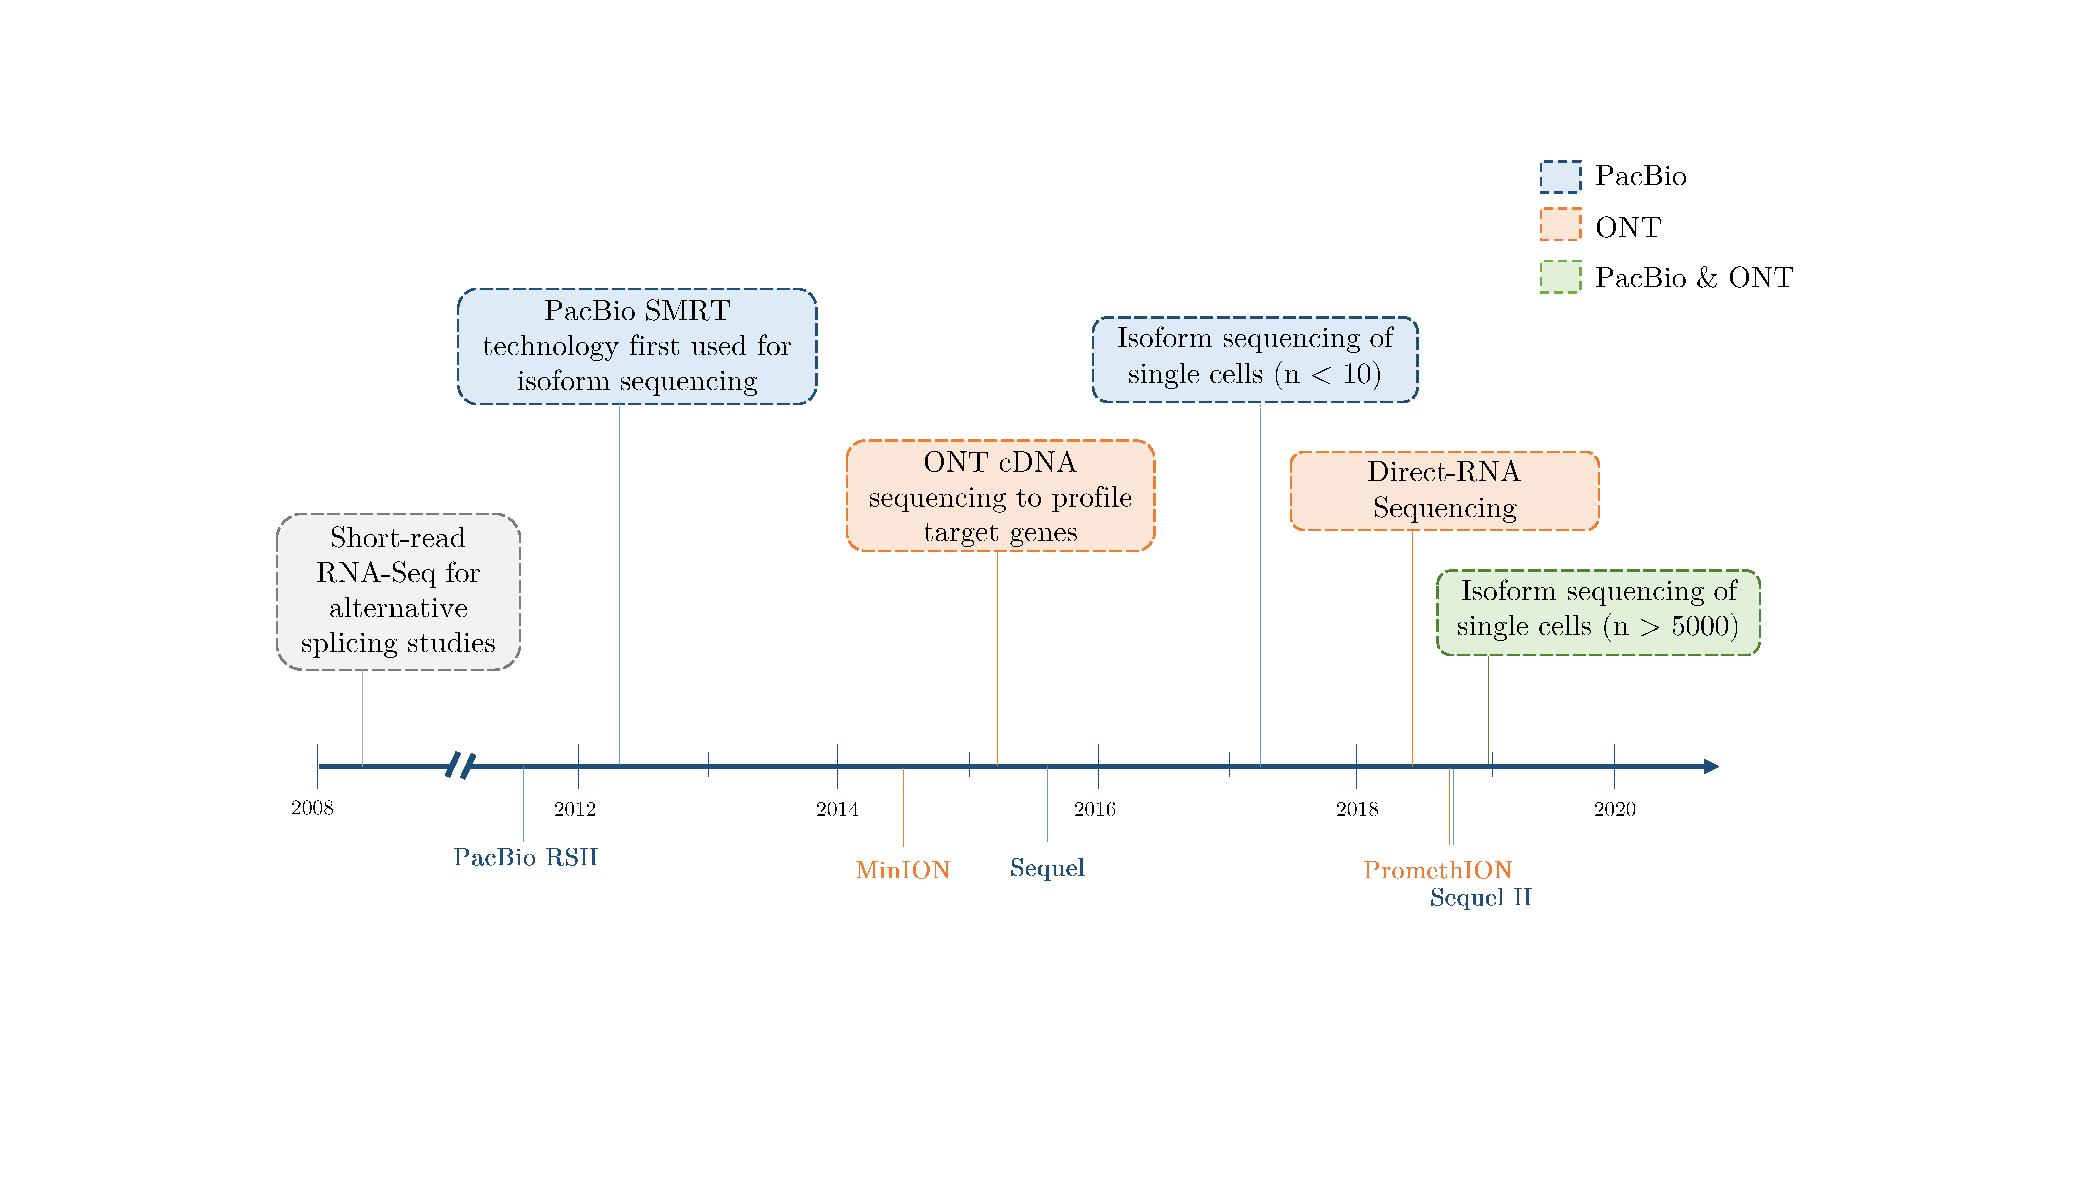
\includegraphics[page=1,trim={0 4cm 1.8cm 2cm},clip, scale = 0.8]{Figures/Introduction_Figures_Landscape.pdf}
			\captionsetup{margin={2cm,0cm}}
			\caption[Timeline of long read sequencing technology \& approaches]%
			{\textbf{Significant advances in long read sequencing technology \& approaches}: Major breakthroughs in long-read sequencing approaches of isoforms using Pacific Bioscience's (PacBio) Single molecule real-time sequencing (SMRT) (boxed blue) and Oxford Nanopore sequencing (ONT, boxed orange) are highlighted. Release of respective technologies are also marked }
			\label{fig:longread_timeline}
		\end{figure}
	\end{landscape}
	
	
	%\captionsetup{width=30cm}
	\begin{landscape}
		\small %smaller font
		\setlength\tabcolsep{2pt} %reduced margin size in table
		\renewcommand{\arraystretch}{1}
		\begin{longtable}[c]{p{4cm}p{4cm}p{18cm}}
			\caption[Long-read sequencing studies of single cells or direct RNA]%		
			{\textbf{Long-read sequencing studies of single cells or direct RNA}, DIE - differential isoform expression}
			\label{tab: longread_advancedstudies}\\
			
			\toprule
			\multicolumn{1}{c}{References} &
			\multicolumn{1}{c}{Samples and Tissue} &
			\multicolumn{1}{c}{Key Findings} \\* \midrule
			\endfirsthead
			%
			\endhead
			%
			\bottomrule
			\endfoot
			%
			\endlastfoot
			%								
			\centering Karlsson \& Linnarsson (2017)\cite{Karlsson2017} &
			\centering Mouse single cels (n = 6)  &
			\tabitem High isoform diveristy observed within single-cell oligodendrocytes with \textasciitilde1000 distinct isoforms mapped to 700 genes with low overlap between cells, predominantly driven by alternative TSS and TTS \\
			\hdashline[0.5pt/5pt]	
			
			\centering Gupta et al.(2018) \cite{Gupta2018} &
			\centering Mouse cerebellum (n = 1)  &
			\tabitem Long-read sequencing of >5000 single cells (microglia, astrocytes, neurons) after isolation \& barcoding \newline 
			\tabitem Identified cell-specific \textit{Bin1} isoforms with skipping of A1 and A2-A6 alternative exons (separated by constitutive exons) in all microglia, some astrocytes but not in neuronal cell-types, indicating cell-specific ES coordination \\
			\hdashline[0.5pt/5pt]			
			
			\centering Byrne et al. (2017)\cite{Byrne2017} &
			\centering Mouse single B1a cells (n = 7) &
			\tabitem Identified thousands of novel TSS and TTS (within 20bp bins due to lower error rate) \& hundreds of splicing events \newline
			\tabitem 160 genes with complex isoforms, 55 of which showed differential isoform usage (including B cell receptors) \\
			\hdashline[0.5pt/5pt]
			
			\centering Volden et al. (2018) \cite{Volden2018} &
			\centering Human single B cells (n = 96 from 1 donor) &
			\tabitem Circularising input cDNA and generating a CCS read (R2C2) significantly improved raw (316,000 cDNA reads at 94\% accuracy) and splice site accuracy (92\% vs ONT 1D raw reads at 80\%, Iso-Seq CCS reads at 97\%, based on SIRVs) \newline 
			\tabitem Ability to accurately demultiplex reads based on 7-8nt barcodes enabling mass sequencing of single cells with accurate gene quantification (strongly correlated with RNA-Seq, r = 0.79) and identification of cell-specific isoforms \\
			\hdashline[0.5pt/5pt]
			
			
			\centering Garalde et al. (2018) \cite{Garalde2018} &
			\centering Yeast \newline ERCC RNA-Spike in mix &
			\tabitem Direct RNA Sequencing of yeast poly(A) RNA achieved good coverage (2.8M reads vs 5.7M reads using ONT cDNA) with negligible effect on transcript length and GC content \newline 
			\tabitem Accurately identification of splice variants with no missing or novel exons from spike-in, and able to rudimentally discriminate RNA modification (m\textsuperscript{6}A, 5-mC) using trained datasets  \\
			
			\centering Workman et al. (2019) \cite{Workman2019a} &
			\centering Human B lymphocyte cell line (n = 30) &
			\tabitem Direct RNA-Sequencing of human cell line documented a high proportion (52.6\%) of novel isoforms \newline
			\tabitem High error rate (14\%) \& significant 5'truncation due to technical issues (rapid translocation through pore, signal artefacts from enzyme stalling or strand breaks), making it difficult to ascertain TSS \newline
			\tabitem Differences in poly(A) length distribution between mitochondrial and nuclear genes, and between different isoforms of the same gene (increase in polyA tail-lengths of intron-retaining isoforms) \\
			\hdashline[0.5pt/5pt]
			
			\centering Sessegolo et al. (2019) \cite{Sessegolo2019} &
			\centering Mouse brain \& liver \newline(n = 3) &
			\tabitem Benchmark study of Illumina RNA-Seq, ONT cDNA-Seq with/without 5'cap, \& ONT Direct RNA-Seq. \newline
			\tabitem Biased ONT cDNA-Seq of truncated transcripts with internal runs of poly(T) (15nt) due to cDNA synthesis; ONT RNA-Seq most accurately quantified gene expression using spike-in, followed by RNA-Seq, cDNA-Seq  \\
			\hdashline[0.5pt/5pt]
			
			\centering Singh et al. (2019) \cite{Singh2019} &
			\centering Human T- \& B-cell lines \newline Tumour \& paired lymph node (n = 1)  &
			\tabitem Novel sequencing method (RAGE-Seq) combining droplet-based scRNA-Seq with target capture ONT cDNA-Seq \newline 
			\tabitem Able to differentiate naive and mature B cells, and subpopulation by accurate identification of antigen receptor; track clonally related cells across tissues revealing cell-specific expression changes between tumour \& lymph node \\
			\hdashline[0.5pt/5pt]
			
			\centering Joglekar et al. 2021 \cite{Joglekar2021} &
			\centering Mouse hippocampus \& prefrontal cortex (n = 2) &
			\tabitem Identified $\tilde{400}$ DIE genes between brain regions using gene-wise test (nx2 table with isoform counts per gene), which was governed predominantly by splice variant changes in one single cell type \newline 
			\tabitem Spatial transcriptomics with Iso-Seq (Sl-ISO-Seq) confirmed localisation of brain-region specific DIE (exon-based). 
			\\* \bottomrule
		\end{longtable}
	\end{landscape}
\end{changemargin}



\newpage
\section{Aims and Objectives}
An increasing number of studies implicate a role of alternative splicing in AD disease development and pathogenesis (reviewed in \cref{tab: AS_ADHuman_studies}). However, such transcriptional profiling studies are typically performed using standard short-read RNA-Sequencing, which is inherently-constrained at transcript assembly and subsequent isoform characterisation essential for splicing analysis (described in \cref{rnaseq_intro}). My PhD thus aims to overcome these challenges by leveraging the use of long-read sequencing to accurately characterise isoform diversity and splicing patterns associated with Alzheimer's disease (\cref{fig:studydesign})

%Further limitations of RNA-Seq studies
%By identifying and characterising such alternative splicing events, there is hope of deepening current understanding of the biological role of transform isoform diversity and in the case of AD, identify novel pathways involved in pathogenesis of disease as potential target treatments. 

\textbf{Hypothesis}: Transcriptomic dysregulation plays a fundamental role in development of AD pathology. This includes alterations in gene splicing, which results in differential and novel expression of transcripts that are translated to generate isoforms with functional biological implications. 

\textbf{Main Objectives}:

\begin{enumerate}[]
	\item Optimise long-read sequencing approaches, PacBio's Iso-Seq and ONT cDNA sequencing, for profiling of full-length transcripts (\cref{ch: long_read_sequencing}) 
	\item Characterise isoform diversity and splicing events in mouse cortex globally using optimised long-read sequencing approaches (\cref{ch: whole_transcriptome}) 
	\item Identify global,age-related transcriptional and splicing changes associated with progression of tau pathology using well-characterised AD mouse model, rTg4510 (\cref{ch: transcriptional_global_differences})
	\item Comprehensively characterise isoform diversity and splicing events of 20 AD-associated genes, and changes in transcript expression associated with tau pathology in rTg4510 mice (\cref{ch: targeted_transcriptome})
	\item Identify AD-associated differential splicing and transcript expression in human post-mortem brain tissue and relate findings to those identified in mouse (\cref{ch: BDR})
	\item Integrate transcriptomic analyses with epigenetic (\cref{ch: targeted_transcriptome}) and proteomic data (\cref{ch: BDR}), available from the same samples
\end{enumerate}
% Integrative Papers
% https://www.nature.com/articles/s41588-020-00773-z importance of linking genomics with proteomics
% https://www.nature.com/articles/s41591-020-0815-6 - more proteomics
% https://www.nature.com/articles/s41588-020-0696-0 - epigenetics


\begin{landscape}
	\begin{figure}[htb]
		\begin{center}
			\includegraphics[page=2,trim={0 0 0 0},clip,scale = 0.7]{Figures/Introduction_Figures_Landscape.pdf}
		\end{center}
		\captionsetup{width=1.5\textwidth}
		\caption[Study design and analysis overview]%
		{\textbf{Study design and analysis overview}. To identify transcriptional and splicing changes associated with AD pathology, this thesis aims to characterise isoform diversity and splicing events at a global and targeted level from the rTg4510 mouse model and AD human post-mortem brain tissues. ONT - Oxford Nanopore Technology, PacBio Iso-Seq - Pacific Bioscience's Isoform Sequencing}
		\label{fig:studydesign}
	\end{figure} 	
\end{landscape}